\documentclass[11pt]{article}
\usepackage[T1]{fontenc}
\usepackage[utf8]{inputenc}
\usepackage[a4paper,margin=24mm]{geometry}
\usepackage{lmodern,microtype}
\usepackage{amsmath,amssymb,amsthm,bm}
\usepackage{graphicx,booktabs,array,tabularx}
\usepackage[small,bf]{caption}
\usepackage[numbers,sort&compress]{natbib}
\usepackage{xcolor}
\usepackage{hyperref}
\usepackage{placeins}
\definecolor{ink}{HTML}{18354A}
\definecolor{accent}{HTML}{177E89}
\hypersetup{colorlinks=true,linkcolor=ink,citecolor=accent,urlcolor=accent}
\setlength{\parskip}{4pt}
\setcounter{tocdepth}{2}
\emergencystretch=2em
\setlength{\parindent}{1em}
\setlength{\textfloatsep}{12pt plus 3pt minus 2pt}
\setlength{\floatsep}{10pt plus 2pt minus 2pt}
\renewcommand{\topfraction}{0.92}
\renewcommand{\bottomfraction}{0.8}
\renewcommand{\textfraction}{0.08}
\newtheorem{proposition}{Proposition}
\newtheorem{corollary}[proposition]{Corollary}
\newcommand{\R}{\mathbb{R}}
\newcommand{\calpha}{C$_\alpha$}
\newcommand{\angstrom}{\text{\AA}}
\newcommand{\Id}{\mathrm{Id}}
\newcommand{\spec}{\operatorname{spec}}
\newcommand{\rank}{\operatorname{rank}}
\newcommand{\im}{\operatorname{im}}
\newcommand{\diag}{\operatorname{diag}}
\newcommand{\del}{\operatorname{del}}
\newcommand{\lk}{\operatorname{lk}}
% The analysis pipeline writes this file. Values are never copied from an old draft.
% Generated by scripts/summarize_study.py; do not transcribe historical metrics here.
\newcommand{\StudyProteins}{364}
\newcommand{\StudyResidues}{78,400}
\newcommand{\StudyClusters}{349}
\newcommand{\GraphPCC}{0.625}
\newcommand{\NativePCC}{0.611}
\newcommand{\NativeGraphPCC}{0.628}
\newcommand{\CenterPCC}{0.565}
\newcommand{\CombinedPCC}{0.627}
\newcommand{\CombinedCILow}{0.613}
\newcommand{\CombinedCIHigh}{0.641}
\newcommand{\DeltaPCC}{+0.0018}
\newcommand{\DeltaCILow}{-0.0009}
\newcommand{\DeltaCIHigh}{+0.0044}
\newcommand{\AbstractEmpiricalResults}{The graph baseline attained mean per-protein correlation $0.625$, while adding corrected center-zero degree-zero spectra yielded $0.627$ (paired difference $+0.0018$; 95\% cluster-bootstrap interval $[-0.0009,+0.0044]$). The primary comparison does not resolve an improvement in mean correlation under this evaluation.}

\newcommand{\paperfigure}[3]{%
\begin{figure}[tbp]\centering
\includegraphics[width=\linewidth]{figures/#1.pdf}
\caption{#2}\label{#3}\end{figure}}

\title{\color{ink}\bfseries Interpreting Local Sheaf Spectra for Protein B-Factor Prediction}
\author{Ryan Charette\\\small The University of Texas at Austin}
\date{}
\begin{document}
\maketitle
\begin{abstract}
A protein structure can be converted into a local graph, enriched with higher-dimensional cells and sheaf comparison maps, and summarized through Laplacian eigenvalues. This manuscript develops that sequence of ideas for readers with a background in linear algebra and then asks what the resulting descriptors measure and whether they improve prediction of relative crystallographic B-factors. Tutorial derivations, worked matrix examples, and the complete experimental record accompany the characterization of two center-labeled constructions and their evaluation under sequence-cluster-held-out validation. A previously used native construction is a weighted contact-graph Laplacian: its universal center introduces an explicit spectral mode, and its largest eigenvalue reduces to neighborhood size. For a rank-one cellular sheaf with a zero center label, the cochain complex separates into a vertex-deletion block and an augmented, geometrically weighted link block. These identities clarify which spectral summaries describe packing, neighbor organization, and local topology. A corrected alpha-complex analysis separates a fixed spatial support from the filtration scale, and a degree-one experiment uses nested pairs of complexes and a Schur-complement persistent operator. \AbstractEmpiricalResults\ Interventional TreeSHAP explanations are computed for held-out proteins using the evaluated model, then mapped to residue coordinates with explicit feature and scale labels. The study provides a mathematical interpretation and controlled empirical assessment of these descriptors. Biological mechanisms require independent evidence, and predictive value must be measured against simpler descriptors. The target remains relative crystallographic B-factor, with the limitations of that observable kept separate from properties of the representation.
\end{abstract}
\vspace{3pt}
\noindent\textbf{Keywords:} cellular sheaves; persistent Laplacians; alpha complexes; protein geometry; B-factors; feature attribution

\clearpage\tableofcontents\clearpage
\section*{How to read this manuscript}
\addcontentsline{toc}{section}{How to read this manuscript}
This manuscript combines a tutorial survey with an original computational study. Its intended reader has graduate-level familiarity with linear algebra, basic probability, and algorithms, but need not have studied algebraic topology, sheaf theory, crystallography, or protein modeling. Familiarity with eigenvalues, least squares, and train--test evaluation is enough to begin. Definitions are developed before they are used in the research analysis, and the extended derivations and experimental details are included in this document.

The central question is deliberately concrete: when a protein neighborhood is converted into a sheaf Laplacian and then into a few eigenvalue statistics, what has been measured, and does that measurement improve prediction of a crystallographic B-factor profile? Answering the first part requires mathematics. Answering the second requires a controlled experiment. Neither answer can substitute for the other.

\paragraph{A route through the argument.}
Part I introduces the biological observable and surveys the existing approaches already cited in this study. Part II builds the mathematical machinery from graph incidence matrices to simplicial cochains and sheaves. Part III develops the specific spectral characterizations and persistent pair operators. Part IV explains the experimental design and reports the unchanged benchmark and attribution results. The final discussion separates what the algebra proves, what the experiment supports, and what remains unknown.

For a first pass, follow the worked examples and the interpretations immediately after the formulas. On a second pass, examine the full derivations and numerical conventions. A reader interested primarily in prediction can read Part I, the graph and sheaf examples in Part II, and then Part IV, returning to the operator derivations when needed. A reader interested primarily in topology should still read the definition of the target and the evaluation design: these determine what a predictive comparison can mean.

\paragraph{Three distinctions to keep in view.}
First, a protein coordinate is an experimental structural input, whereas a cochain coordinate is an abstract variable on a vertex, edge, or triangle. Second, a zero eigenvalue has a cohomological interpretation, whereas a positive eigenvalue also depends on geometric weights and inner products. Third, a model attribution explains a fitted predictor, whereas an incremental performance comparison asks whether adding features helps that predictor on held-out data. Many apparent paradoxes disappear once these objects are kept separate.

\clearpage
\subsection*{Notation at a glance}
\begin{center}\small
\begin{tabularx}{\linewidth}{lX}\toprule
Symbol & Meaning in this manuscript\\\midrule
$p,i$ & Protein entry and retained residue index, when used in target notation.\\
$x_i\in\R^3$ & Observed C-alpha coordinate of residue $i$.\\
$c,\ P_c,\ R$ & Target residue, its fixed coordinate neighborhood, and support radius.\\
$a\leq b,\ K_a\subseteq K_b$ & Alpha radii and their nested simplicial complexes.\\
$\sigma,\tau$ & Simplices, with $\sigma\subseteq\tau$ a face relation.\\
$q$ & Cochain degree: vertices at degree zero, edges at degree one.\\
$q_v$ & A vertex label in the restriction rule; the subscript distinguishes it from degree.\\
$\rho_{\sigma\tau}$ & Linear comparison map from the stalk on a face to its coface.\\
$C^q,\ d_q,\ D_q$ & Cochain space, coboundary map, and its matrix in an oriented basis.\\
$L_q,\ L_q^{a,b}$ & Ordinary and persistent sheaf Laplacians.\\
$\beta_q,\widetilde\beta_q$ & Ordinary and reduced Betti numbers, respectively.\\
$B_{ip},\ y_{ip}$ & Measured B-factor and its within-protein standardized value.\\
$f(x),\phi_j(x)$ & Model prediction and attribution of feature $j$; here $x$ is a feature vector.\\\bottomrule
\end{tabularx}
\end{center}
The same letter can occur in separate, explicitly identified contexts. In particular, the block $B$ in a matrix partition is not a crystallographic B-factor, and the historical native parameter $p$ is not a protein index. In the matrix derivations, a superscript $T$ denotes transpose and $\dagger$ denotes the Moore--Penrose pseudoinverse. Unless stated otherwise, cochain coordinates have the standard Euclidean inner product, so transpose is also the adjoint.

\paragraph{Status of the material.}
The background and worked examples explain established constructions. The research contribution is the interpretation of the specified local operators and their controlled assessment on the audited collection. The expanded exposition does not introduce a new benchmark, a new parameter search, or additional empirical claims. The numerical results are the same generated results used in the shorter research article.

\clearpage\part{The problem and its scientific context}
\section{Introduction}
Protein structures are commonly represented as lists of atomic coordinates, yet many useful questions concern relationships: which residues constrain one another, how a neighborhood is organized, and which parts of a molecule have comparatively high positional disorder. A contact count describes one aspect of those relationships. A graph spectrum describes a richer arrangement of contacts. A cellular sheaf adds a rule for comparing local assignments across cells, while a filtration records how a representation changes as a geometric scale is varied. Each additional construction introduces mathematical structure. Whether it introduces additional information relevant to a biological target is an empirical question.

Crystallographic B-factors provide a practical setting in which to examine that question. Elastic-network models connect residue contacts to collective fluctuations through graph-based operators \citep{haliloglu1997,atilgan2001}. Flexibility--rigidity indices use distance-dependent neighborhood interactions \citep{nguyen2016}. Persistent homology and related spectral methods describe molecular organization across scales \citep{xia2014,wang2020}. Each approach must specify how its geometric construction defines the measured quantity. In particular, a feature computed from a matrix called a sheaf Laplacian can behave like a familiar packing statistic under a particular choice of labels and neighborhood.

The present work began with a research implementation for local persistent sheaf Laplacian (PSL) descriptors and B-factor prediction. Examining the native computational path revealed a distinction between two operations that had been grouped under that terminology. One increases contact-edge weights when vertex labels differ; the other places vertex labels in face-to-coface restriction maps. For a zero-labeled center, the former strengthens center--neighbor coupling and the latter removes an entire class of couplings. These constructions cannot support the same mathematical interpretation. Moreover, changing edge weights with a parameter is different from computing a persistent operator for a pair of nested complexes. This distinction motivates treating the existing native descriptor as an explicit graph baseline and analyzing a separately specified sheaf construction.

Three questions organize the study. First, what parts of the local geometry can be read directly from each operator? Second, do the corresponding spectral summaries add predictive information beyond a predefined collection of simple graph and packing features when detected related protein sequences are held out together? Third, does degree-one persistence supply information beyond that available from degree-zero spectra and endpoint scales? A mathematical reduction, a well-supported null comparison, and a localized explanation of when a descriptor succeeds or fails can each clarify its scientific value.

We combine an operator audit with controlled experiments and residue-level visualization. The mathematical analysis establishes an explicit spectrum for the native universal-center graph and a block decomposition for the zero-centered sheaf. The latter specializes established weighted-complex and sheaf constructions to explain this application. The experiments distinguish identity, geometric, and center-zero restrictions; use a common prediction model; and evaluate incremental performance on the same held-out proteins. The visual analysis follows the same separation: observed B-factor, predicted B-factor, and signed model contributions appear as distinct quantities on the same structure.

\paperfigure{fig1_protein}{The predetermined principal protein 1ULR. (a,b) Observed within-protein normalized B-factor and the held-out graph-plus-center-zero prediction on the same structure and color scale. (c) The signed sum of TreeSHAP contributions from the 24 center-zero spectral features, excluding graph contributions and the background expectation. Blue contributions lower and red contributions raise this model's output. (d) Observed and predicted residue profiles show agreement and local errors. (e) The alpha complex at radius 4~\AA\ within the fixed 13~\AA\ support of chain A residue 43. Attributions describe how the evaluated model uses features of the target residue. They require a separate interpretation from experimental measurements or neighboring-residue effects.}{fig:protein}

\section{A minimal structural-biology vocabulary}
A protein is built from amino-acid residues connected along one or more chains. A residue contains several atoms; the C-alpha atom supplies one convenient reference point for its position along the backbone. Replacing a structure by its C-alpha coordinates produces a point cloud that retains the coarse arrangement of the resolved chain while discarding most atomic detail. An edge in a geometric graph on this cloud indicates a chosen spatial relationship. It need not be a covalent bond, and residues close in three-dimensional space need not be adjacent in sequence.

A deposited coordinate model is also not a movie. The crystallographic B-factor attached to an atom is an atomic displacement parameter, interpreted within the structure-determination model. It can be influenced by motion and disorder, but the coordinate file alone does not separate those contributions. This is why the study predicts a stated crystallographic observable rather than claiming to recover solution trajectories. The formula relating B-factors to isotropic displacement appears in the next section; the experimental outcome below is further standardized within each protein.

The three views in Figure~\ref{fig:protein} can now be read without knowing any sheaf theory. The first is the measured relative profile mapped to the structure. The second is a prediction for a protein excluded from that model's training groups. Their common color scale permits a direct visual comparison. The third uses a different scale because it shows only the signed contribution of one feature family to the prediction. A warm region in that panel says that this group raises the fitted model's output relative to its background expectation. It does not say that a sheaf feature causes motion at that residue.


\section{Related work and the prediction target}
\subsection{Crystallographic displacement and geometric prediction}
For an isotropic atomic displacement parameter $U_{\mathrm{iso}}$, the crystallographic convention is $B=8\pi^2 U_{\mathrm{iso}}$. If $u$ denotes a three-dimensional isotropic displacement vector, then $U_{\mathrm{iso}}=\mathbb{E}\|u\|^2/3$. The definition of displacement therefore matters when converting between B-factors and fluctuation amplitudes. B-factors also reflect static disorder and aspects of structure determination, including refinement, occupancy, resolution, and crystal packing. Their normalization is consequential when comparing structures \citep{carugo2018}. We use the term flexibility as a motivation for the task, while defining the actual response as a within-protein B-factor profile.

Geometry-based models have a long history in this setting. The Gaussian network model uses a contact-network Laplacian and its inverse-mode structure to describe equilibrium fluctuations \citep{haliloglu1997}; the anisotropic network model retains direction-dependent information \citep{atilgan2001}. Kernel-based rigidity descriptors aggregate nearby interactions without requiring a hard contact cutoff \citep{nguyen2016}. Graphlet-based work also demonstrates that local graph organization is a meaningful comparator for atomic displacement prediction \citep{praznikar2023}. Our graph baseline uses simple structural summaries in a supervised predictor. Elastic-network dynamical models address a different modeling task. Comparing this baseline with PSL descriptors isolates a representation question under the same regressor.

Feng and colleagues developed multiscale differential-geometric descriptors and released the structural collection used here \citep{feng2025}. Their use of curvature has a specific differential-geometric definition. We call the eigenvalue statistics in this paper spectral summaries. Their definitions differ from sectional, Gaussian, mean, and discrete Ricci curvature. Hayes and colleagues applied persistent sheaf Laplacians to protein B-factors \citep{hayes2025}. The original reported average comparison with the Gaussian network model was 32\%; a correction of a dataset-aggregation error revised it to 20\% \citep{hayes2025correction}. Both percentages belong to that earlier study; we use its corrected record. An extension to protein--nucleic-acid complexes \citep{hayes2026} and an application to mutation-associated stability and solubility \citep{ren2026} establish a broader context for PSL-based molecular descriptors, with different targets and evaluation protocols.

\subsection{Sheaf theory and local spectra}
Spectral sheaf theory relates cellular cohomology to positive-semidefinite Laplacians \citep{hansen2019}. A sheaf specifies vector spaces on cells and compatible linear maps across face relations. It is the compatibility of these maps, together with the cell incidence signs and chosen inner products, that supports a cochain complex and a Hodge-type interpretation. Weighted boundary operators provide a related perspective, including the effects of vanishing vertex weights \citep{renwu2021}. Wei and Wei extend the spectral construction to pairs of sheaves on nested complexes and supply geometric rank-one examples \citep{wei2025}.

Persistent Laplacians have their own algorithmic foundations. M\'emoli, Wan, and Wang develop Schur-complement formulations and analyze their relation to persistent Betti numbers \citep{memoli2022}. Our numerical construction uses that linear-algebraic principle in the sheaf cochain setting. Related empirical work evaluates higher-order persistent spectral representations across data-science problems \citep{davies2023}; their predictive value can be assessed through controlled comparisons at different degrees.

Local topology is also connected classically to vertex links. A recent preprint of Liu, Feng, and Liu develops local Laplacians and identifies a persistent local operator with a shifted-degree link operator \citep{liu2026}. Our center-zero decomposition should be read alongside that work: it retains both a deletion contribution and an augmented link contribution, with the geometric weights inherited from the specified restriction maps. The application-level question is which of these contributions a residue descriptor contains and whether it helps explain B-factor variation. We make no priority claim for deletion/link decompositions or for local persistent spectral analysis in general.

\subsection{What an explanation explains}
SHAP values allocate a model output among input features under a specified coalition value function \citep{lundberg2017}. TreeSHAP makes these calculations practical for tree ensembles \citep{lundberg2020}. An explanation is consequently conditional on the trained model, input representation, and background distribution. Correlated geometric features may divide credit between alternative summaries of the same environment. The feature combinations used by this attribution game can lie outside the set realizable by atomic coordinates. SHAP describes model behavior and permits comparisons by geometric scale. Molecular causation requires independent evidence.

\subsection{A map of the existing approaches}
The methods surveyed here differ both in how they represent a structure and in how they turn that representation into a prediction. Keeping those decisions separate is useful when reading the literature. An elastic-network model gives its operator a physical interpretation under modeling assumptions. A supervised descriptor pipeline can use a related matrix simply as a source of input features. Similar-looking matrices therefore need not imply identical scientific claims.

\begin{table}[htbp]\centering\small
\caption{Conceptual map of the approaches discussed in the cited literature. This is a guide to their roles, not a new comparison of predictive accuracy.}
\begin{tabularx}{\linewidth}{>{\raggedright\arraybackslash}p{.23\linewidth}>{\raggedright\arraybackslash}X>{\raggedright\arraybackslash}X}\toprule
Approach & Structural representation & Quantity emphasized\\\midrule
Elastic networks & A residue contact network, with scalar or direction-dependent interactions & Collective fluctuation modes under the network model \citep{haliloglu1997,atilgan2001}.\\
Flexibility--rigidity indices & Distance-dependent sums around atoms or residues & Local interaction density across selected kernels and scales \citep{nguyen2016}.\\
Graph organization & Contacts and small graph configurations & The arrangement of contacts beyond a single count \citep{praznikar2023}.\\
Persistent homology & A nested family of complexes & The appearance and disappearance of topological classes \citep{xia2014}.\\
Persistent Laplacians & Operators associated with pairs of nested complexes & Kernel information together with positive spectral information \citep{wang2020,memoli2022,davies2023}.\\
Cellular sheaf spectra & Cellwise vector spaces and compatible comparison maps & Cohomology and weighted disagreement of local assignments \citep{hansen2019,wei2025}.\\\bottomrule
\end{tabularx}
\end{table}

Three successive questions organize this progression. Which points should interact? Which higher-dimensional cells should be included? How should assignments on different cells be compared? A contact graph answers the first question. A simplicial complex also answers the second. A cellular sheaf supplies the third ingredient. Persistence then asks how a compatible construction behaves across two members of a nested family. These choices are independent enough that they should be stated explicitly rather than hidden in a descriptor's name.

The distinction between geometry and topology will recur throughout the manuscript. Geometry includes distances, angles, and weights. Topology concerns connectivity and higher-dimensional holes, as represented by the chosen complex. Changing distances can alter a positive eigenvalue even when the complex and its Betti numbers stay unchanged. Conversely, adding a triangle can remove a one-dimensional topological class without changing any vertex or edge. A spectral representation can contain both kinds of information, but it should not call every spectral change a topological change.

The controlled comparison in this work places these representations inside one fixed learning setup. It asks whether the chosen summaries add useful predictive information beyond a specified geometric baseline. It does not compare optimized implementations of every method in the table. This narrower question makes it possible to connect the empirical outcome to the detailed operator analysis that follows.

\FloatBarrier\clearpage\part{Mathematical foundations}
\section{Graphs, cochains, and Laplacians}
\label{sec:foundations}
\subsection{Incidence matrices turn local differences into linear algebra}
Begin with an undirected graph whose vertices are residues and whose edges are selected contacts. Assign a real number $z_i$ to every vertex. At this stage $z$ is an arbitrary test assignment used to examine the operator. Give each edge an arbitrary orientation solely to define a matrix. The row of the incidence matrix $D_0$ associated with an oriented edge $i\to j$ contains $-1$ in column $i$, $+1$ in column $j$, and zeros elsewhere. Then $(D_0z)_{ij}=z_j-z_i$.

The graph Laplacian is $L_0=D_0^TD_0$. For nonnegative edge weights $w_{ij}$, replace each incidence row by $\sqrt{w_{ij}}$ times that row. In either case,
\begin{equation}
z^TL_0z=\|D_0z\|^2=\sum_{ij}w_{ij}(z_j-z_i)^2.
\label{eq:graph-tutorial-energy}
\end{equation}
The matrix measures a sum of local disagreements. Reversing one edge changes the sign of a row of $D_0$ but does not change $D_0^TD_0$. Thus the arbitrary orientation does not become a physical direction of interaction. This elementary observation is the starting point for orientation invariance in the more general construction.

If all graph weights are positive, the energy is zero exactly when the assignment is constant on each connected component. A connected graph therefore has a one-dimensional kernel, spanned by the all-ones vector. If the graph has several components, one constant can be chosen independently on each. This explains the familiar equality between graph-Laplacian nullity and component count without appealing to topology terminology.

\subsection{What an eigenvalue measures}
Because $L_0$ is real symmetric, it has an orthonormal eigenbasis. Write a unit-norm assignment as $z=\sum_k\alpha_kv_k$, with $L_0v_k=\lambda_kv_k$. Its energy is $\sum_k\lambda_k\alpha_k^2$. A small positive eigenvalue identifies a direction of low disagreement relative to the chosen norm; a large eigenvalue identifies a direction of higher disagreement. Multiplying every edge weight by a positive constant multiplies every eigenvalue by that constant while leaving the graph's connectivity unchanged.

Consequently, the kernel and positive spectrum answer different questions. Kernel dimension records exact zero-energy freedoms. Positive eigenvalues measure the scale of nonzero disagreement and depend on the weights and inner product. In this manuscript, eigenvalues become descriptors only after they have been summarized. The learner does not receive the full eigenvectors, so a good prediction from spectral summaries is not itself evidence that a particular eigenvector describes a molecular motion.

\subsection{The triangular outline and its filling}
A simplicial complex extends a graph by specifying which collections of vertices form higher-dimensional cells. A vertex is a zero-simplex, an edge a one-simplex, and a filled triangle a two-simplex. A tetrahedron is a three-simplex. Every face of an included simplex must also be included. Three edges forming a triangular outline and the same three edges together with a filled triangle are different complexes, although their contact graphs are identical.

To see the distinction as linear algebra, order the vertices as $0,1,2$ and edges as $01,02,12$. For either complex the vertex-to-edge matrix is
\begin{equation}
D_0=\begin{pmatrix}-1&1&0\\-1&0&1\\0&-1&1\end{pmatrix}.
\end{equation}
If the triangle is filled, the edge-to-triangle matrix is $D_1=(1,-1,1)$. Its action on edge values $w$ is $w_{01}-w_{02}+w_{12}$, the signed circulation around the triangle. Multiplication gives $D_1D_0=0$: differences of vertex values have zero circulation. If the triangle is not filled, there is no triangle row and $D_1$ is the zero map into a zero-dimensional space.

\subsection{Cochains, cocycles, and the quotient called cohomology}
A \emph{cochain} is simply an assignment to cells of one dimension: vertex values at degree zero, edge values at degree one, and triangle values at degree two. The vector space of these assignments is denoted $C^q$. A \emph{coboundary map} $d_q:C^q\to C^{q+1}$ compares an assignment around the next-dimensional cells. Its matrix is $D_q$. The identity $d_{q+1}d_q=0$ says that applying two consecutive comparisons gives zero.

A \emph{cocycle} lies in $\ker d_q$. A \emph{coboundary} lies in $\im d_{q-1}$, meaning that it came from an assignment one degree below. Every coboundary is a cocycle because consecutive maps compose to zero. Cohomology is the quotient
\begin{equation}
H^q=\ker d_q/\im d_{q-1}.
\label{eq:tutorial-cohomology}
\end{equation}
The quotient identifies cocycles that differ only by a coboundary. It measures zero-comparison assignments that cannot be explained entirely as differences of lower-degree assignments. This is a vector-space construction: one can compute its dimension using ranks, without first developing general algebraic topology.

For ordinary real cochains, $\dim H^q$ is the Betti number $\beta_q$. In low dimensions, $\beta_0$ counts connected components and $\beta_1$ counts independent cycles not filled by two-dimensional cells. We use cohomology because face-to-coface comparison maps naturally produce cochains. Over the real numbers its ordinary dimensions agree with those obtained from homology, whose boundary maps run in the opposite direction. The map direction matters again when a pair of complexes is considered.

\subsection{The Hodge Laplacian selects representatives of cohomology}
With Euclidean inner products, define
\begin{equation}
L_q=D_q^TD_q+D_{q-1}D_{q-1}^T.
\end{equation}
For an assignment $w$, its quadratic form is $\|D_qw\|^2+\|D_{q-1}^Tw\|^2$. Therefore $w$ lies in the kernel precisely when it is a cocycle and is orthogonal to every coboundary. Such a vector is called \emph{harmonic}. Here the word describes these two linear conditions.

Why does every cohomology class have exactly one harmonic representative? Start with a cocycle and subtract its orthogonal projection onto $\im d_{q-1}$. The remainder stays a cocycle, since the subtracted vector is also a cocycle, and is orthogonal to all coboundaries. Two such remainders representing the same class would differ by a vector both in and orthogonal to $\im d_{q-1}$; that difference must be zero. This proves the kernel interpretation by finite-dimensional linear algebra. Cellular sheaf Laplacians use the same argument once their maps satisfy the cochain identity \citep{hansen2019}.

Return to the triangle. For its unfilled outline, $h=(1,-1,1)^T$ satisfies $D_0^Th=0$ and is a nonzero harmonic edge assignment. Thus the edge Laplacian has a one-dimensional kernel. Filling the triangle adds $D_1^TD_1=hh^T$. Direct multiplication gives
\begin{equation}
L_1^{\mathrm{outline}}=D_0D_0^T,
\qquad L_1^{\mathrm{filled}}=D_0D_0^T+hh^T=3I_3.
\end{equation}
The outline has edge spectrum $\{0,3,3\}$, whereas the filled triangle has $\{3,3,3\}$. Both have the same vertex spectrum $\{0,3,3\}$. A degree-one operator can therefore distinguish a filling that a degree-zero graph operator cannot see. These exact matrices illustrate the definitions.

\subsection{Geometric filtrations}
A filtration is a nested sequence of complexes: a cell, once included, stays included as the parameter increases. One simple construction connects all pairs at distance below a threshold and includes every clique as a simplex; this is a Vietoris--Rips construction. An alpha complex uses the geometry of a Delaunay triangulation and restricted balls. The radius convention and the rule for including higher-dimensional cells must therefore be specified explicitly.

For intuition about alpha complexes, associate each point with its Voronoi region, consisting of locations at least as close to that point as to any other. Intersect a radius-$a$ ball around each point with its Voronoi region. The alpha complex encodes common intersections of these restricted regions through simplices in the Delaunay structure \citep{edelsbrunner1994,gudhi}. This produces a finite geometric representation of the growing union of balls. The radius parameter specifies the size of these balls.

With only two points at distance $d$, the balls first meet at $a=d/2$. With more points, Voronoi restrictions also matter, so an arbitrary pair within distance $2a$ is not automatically an alpha edge. The code uses this alpha-complex construction directly. GUDHI stores squared filtration radii; the manuscript reports the unsquared radii in angstroms.

A final distinction concerns which points are allowed to enter this construction. The support radius $R$ first fixes the residue neighborhood. The alpha radius $a$ then changes the cells within that same point set. Keeping $R$ fixed holds the residue sample constant while $a$ varies the filtration. The next section specifies both choices for the protein descriptors.

\section{Local complexes and cellular sheaves}
\subsection{Two geometric scales}
Let $P=\{x_1,\ldots,x_n\}\subset\R^3$ be the observed \calpha\ coordinates in an analyzed structure, and let $c$ denote a target residue. The corrected representation first selects the fixed support
\begin{equation}
P_c=\{x_j:\|x_j-x_c\|\leq R\},\qquad R=13\,\angstrom.
\label{eq:support}
\end{equation}
Within this point set, $K_a$ is the alpha complex at ball radius $a$. Alpha complexes are subcomplexes of a Delaunay triangulation and describe the union of restricted balls through a finite simplicial representation \citep{edelsbrunner1994}. All vertices of $P_c$ are present at the nonnegative scales considered here, and $K_a\subseteq K_b$ for $a\leq b$. The support radius chooses which residues can participate; the alpha radius chooses which simplices appear among those residues. Varying them together would confound two different operations.

An oriented $q$-simplex is written $\sigma=[v_0,\ldots,v_q]$, using a fixed vertex ordering. A face is obtained by deleting vertices, and a simplicial complex contains every face of each of its simplices. The incidence number $[\sigma:\tau]$ for a codimension-one face is the sign of the corresponding deletion. These signs ensure cancellation when two consecutive coboundaries are composed. For implementation, GUDHI alpha values are squared radii \citep{gudhi}; a filtration threshold $a$ in angstroms is therefore implemented at $a^2$. This is independent of the edge-length scale introduced below.

\subsection{What a sheaf adds to the complex}
The incidence matrix compares vertex values by ordinary subtraction. A cellular sheaf generalizes the comparison rule. It attaches a vector space, called a \emph{stalk}, to every cell, and specifies linear maps between the spaces on faces and cofaces. To compare values from two vertices, first map them into the common edge space and then subtract. The maps define how the cellwise assignments are compared.

In the present study every stalk is $\R$. Thus all stalk values are scalars and all comparison maps are multiplication by real numbers. The phrase \emph{rank-one sheaf} refers to the dimension of each stalk. A neighborhood with many vertices can still produce a large, high-rank matrix. The more general theory permits different vector-space dimensions and matrix-valued maps, but those possibilities are not needed here \citep{hansen2019}.

The maps are traditionally called restrictions. Our convention uses the face's stalk as the domain and the coface's stalk as the codomain. The displayed arrow $\rho_{\sigma\tau}:\mathcal S(\sigma)\to\mathcal S(\tau)$ specifies the direction. All formulas in this manuscript use this convention consistently.

Why impose compatibility? Suppose a vertex belongs to a triangle through two different intervening edges. The value obtained by mapping the vertex assignment to the triangle must agree along both routes. Otherwise the cancellation in the triangle calculation above can fail. Compatibility guarantees that the two routes have the same map; the incidence signs give them opposite signs. The identity $d_{q+1}d_q=0$ then follows. An arbitrary collection of edge weights can define a positive-semidefinite graph Laplacian without satisfying this stronger higher-dimensional requirement.

It is helpful to separate three ingredients. The complex says which cells exist. The restriction maps say how assignments are compared. The inner products say how large an assignment or a disagreement is. Changing any of these can change a Laplacian. A statement that two constructions have the same cohomology need not imply that they have the same positive spectrum, because cohomology forgets the size information supplied by the inner products.

\subsection{Reading the geometric restriction rule}
The restriction formula multiplies a ratio of positive geometric factors by the labels of newly added vertices. For a vertex the geometric factor is one. For an edge it is its dimensionless length. For a triangle it is the product of its three edge lengths. For an edge contained in a triangle, the restriction divides by the two additional edge lengths and multiplies by the label of the newly added vertex.

Following two successive face relations multiplies two ratios whose intermediate factors cancel. The label products similarly combine into the labels of all newly added vertices. This telescoping is the mechanism behind compatibility. A zero label is safe because it appears only in a product, never in a denominator. Coincident points are different: they would introduce zero geometric denominators and must be handled by the coordinate audit.

We use two choices of vertex labels. All-one labels keep the geometric factors. A zero at the target distinguishes the target algebraically from its neighbors. Both choices use only the target identity and geometry. The sheaf is built before fitting the model, so the eventual response cannot influence its restrictions.

\subsection{Restriction maps and the energy of an assignment}
A rank-one cellular sheaf $\mathcal S$ attaches $\R$ to each simplex. For $\sigma\subseteq\tau$, write $\rho_{\sigma\tau}:\mathcal S(\sigma)\to\mathcal S(\tau)$ for the restriction map. The maps satisfy $\rho_{\tau\upsilon}\rho_{\sigma\tau}=\rho_{\sigma\upsilon}$ and $\rho_{\sigma\sigma}=\Id$. In the geometric family, let $q_v$ be a vertex label and define
\begin{equation}
F(\sigma)=\prod_{\{u,v\}\subseteq\sigma}\frac{\|x_u-x_v\|}{\ell_0},\qquad
\rho_{\sigma\tau}=\frac{F(\sigma)}{F(\tau)}\prod_{v\in\tau\setminus\sigma}q_v,
\quad \ell_0=1\,\angstrom.
\label{eq:restrictions}
\end{equation}
The empty product gives $F(v)=1$. Distinct coordinate points make $F$ positive, and the length reference makes its values dimensionless. Both the geometric ratios and label products telescope under composition. Zero labels are allowed because no label is divided out. The construction follows the rank-one family of \citet{wei2025}; choosing a zero center has a specific algebraic effect examined below.

We compare three sheaves on the same alpha complexes. The \emph{identity} sheaf has every restriction equal to one. The \emph{geometric} sheaf uses Equation~\eqref{eq:restrictions} with all $q_v=1$. The \emph{center-zero} sheaf uses $q_c=0$ and $q_v=1$ for $v\ne c$. Identity restrictions and constant vertex labels are distinct choices: the latter still retain distance-dependent factors. These labels mark a distinguished residue. They have no assigned physical charge interpretation.

The cochain space $C^q(K;\mathcal S)=\bigoplus_{\dim\sigma=q}\mathcal S(\sigma)$ contains one scalar per $q$-simplex. In the orthonormal simplex bases used numerically,
\begin{equation}
(d_q z)_\tau=\sum_{\substack{\sigma\subset\tau\\\dim\sigma=q}}[\sigma:\tau]\rho_{\sigma\tau}z_\sigma,
\qquad d_{q+1}d_q=0.
\label{eq:coboundary}
\end{equation}
For an edge $[u,v]$, its degree-zero row is $(-q_v/r_{uv},q_u/r_{uv})$, where $r_{uv}=\|x_u-x_v\|/\ell_0$. Thus
\begin{equation}
z^T L_0 z=\|d_0z\|^2
=\sum_{[u,v]\in K}\frac{(q_u z_v-q_v z_u)^2}{r_{uv}^2},
\qquad L_0=d_0^T d_0.
\label{eq:energy}
\end{equation}
This energy quantifies disagreement of sheaf assignments. A physical elastic interpretation would require additional modeling assumptions. If both labels equal one, it is the energy of an inverse-square-weighted graph. If $q_c=0$, an edge $[c,v]$ contributes $z_c^2/r_{cv}^2$ and contains no cross-term involving $z_v$. A zero label leaves the residue in the point cloud and changes its algebraic couplings. Mechanical rigidity would require a physical model.

In general,
\begin{equation}
L_q=d_q^Td_q+d_{q-1}d_{q-1}^T,
\qquad d_{-1}=0.
\label{eq:laplacian}
\end{equation}
Positive semidefiniteness follows from the sum of two squared norms. Its kernel is the intersection of the cocycle space with the orthogonal complement of coboundaries and represents sheaf cohomology \citep{hansen2019}. Identity-sheaf nullities recover ordinary Betti numbers. Other restrictions require the corresponding sheaf interpretation; zero eigenvalues must not automatically be called connected components or loops of the underlying unweighted complex.

\subsection{A two-vertex example: labeling is not deletion}
Consider one edge of length $2\,\angstrom$, oriented from the target $c$ to its neighbor $v$. With all-one geometric labels, the coboundary and Laplacian are
\begin{equation}
D_0=(-1/2,1/2),\qquad
L_0=\frac14\begin{pmatrix}1&-1\\-1&1\end{pmatrix}.
\end{equation}
Their energy is $(z_v-z_c)^2/4$, and the eigenvalues are $0$ and $1/2$. The zero-energy assignment is constant on the two vertices.

Set the center label to zero while retaining the neighbor label one. The same edge now has
\begin{equation}
D_0=(-1/2,0),\qquad L_0=\begin{pmatrix}1/4&0\\0&0\end{pmatrix}.
\end{equation}
The energy is $z_c^2/4$. It penalizes the center coordinate but imposes no condition on the neighbor coordinate. Both vertices and the edge still exist. The kernel is now spanned by $(0,1)^T$, rather than by the constant assignment. This example explains why it would be incorrect to describe a zero center label as simply removing the target or fixing a measured physical displacement.

It also exposes the contrast with the historical native rule. Increasing the center-edge weight in an ordinary graph strengthens the disagreement penalty between the two endpoints. The center-zero restriction instead removes the cross-term between them. Both constructions yield positive-semidefinite matrices, but they encode different comparisons. Positive semidefiniteness alone cannot establish that an implementation realizes the intended sheaf.

\subsection{Equal topology does not imply equal positive spectra}
For all-one geometric restrictions, an invertible rescaling of cochain coordinates can transform the coboundary maps into ordinary incidence maps. This is often called a \emph{gauge change}. Invertibility preserves kernels and images up to isomorphism, so the cohomology dimensions agree. It does not generally preserve the Euclidean length of vectors. The transformed adjoint is therefore not obtained by merely applying the same change to a matrix transpose.

The two-vertex example already demonstrates the issue: the unweighted edge Laplacian has eigenvalues $0$ and $2$, while the length-two geometric edge has eigenvalues $0$ and $1/2$. Their complexes and cohomology agree, but their positive spectra differ. An orthogonal change of basis would preserve eigenvalues; a general diagonal rescaling need not. Later, this distinction explains why identity and geometric sheaves have matching nullities while still supplying different positive-spectrum features.

\paragraph{What reaches the predictor.}
For each residue and each declared scale, the operator is reduced to six numbers: nullity and five summaries of its positive eigenvalues. These features are not the cochain assignment $z$ used to define energy. They are measurements of the operator itself. The same construction is repeated with each retained residue as the target, giving one feature row per residue. Only then is a forest trained to relate those rows to standardized B-factors.

\paperfigure{fig2_pipeline}{Local spectral descriptor construction. (a) The fixed 13~\AA\ support around residue 43 of chain A in 1ULR contains 41 \calpha\ vertices; red identifies the center. (b,c) Alpha complexes at ball radii 3 and 4~\AA\ retain those vertices while adding edges and triangles. (d) Compatible center-zero restrictions define a cochain complex. The figure's $d_{ij}=\|x_i-x_j\|/(1~\angstrom)$ is the dimensionless distance denoted $r_{ij}$ in the text. (e) The degree-zero center-zero Laplacian at $a=4$~\AA, with local-vertex indices on both axes. (f) Ordered eigenvalues at the two scales. These are geometric operators and spectra, prior to fitting a B-factor model.}{fig:pipeline}

\FloatBarrier\clearpage\part{Interpreting the specified local operators}
\section{What the local spectra contain}
\subsection{The native descriptor is a universal-center graph}
The retained native descriptor builds a distance-threshold graph on a neighborhood of radius $r$, using the same $r$ as the edge cutoff. The center is consequently adjacent to every selected neighbor. At its evaluated parameter value $p=0$, an edge has weight $1+|q_u-q_v|$. Center-zero labeling gives weight two on center edges and weight one on edges between neighbors. Let $H$ be this neighbor-induced unweighted graph, with $m$ vertices and Laplacian $L_H$. For $m\geq1$, the native matrix is
\begin{equation}
L_{\mathrm{native}}=
\begin{pmatrix}2m&-2\mathbf1^T\\-2\mathbf1&L_H+2I_m\end{pmatrix}.
\label{eq:native}
\end{equation}
It is a valid weighted graph Laplacian, but it is different from Equation~\eqref{eq:energy}. This classification applies to the inspected implementation.

\begin{proposition}[Native spectrum]
If $0=\lambda_1\leq\lambda_2\leq\cdots\leq\lambda_m$ is the spectrum of $L_H$, counting all zero eigenvalues, then
\begin{equation}
\spec(L_{\mathrm{native}})=\{0,2(m+1)\}\cup\{\lambda_j+2:2\leq j\leq m\}.
\label{eq:native-spectrum}
\end{equation}
The native nullity is one and its largest eigenvalue is $2(m+1)$.
\label{prop:native}
\end{proposition}
\begin{proof}
The all-ones vector is in the kernel. The vector $(m,-\mathbf1)^T$ is an eigenvector with eigenvalue $2(m+1)$. Every neighbor vector $v\perp\mathbf1$ satisfying $L_Hv=\lambda v$ lifts to $(0,v)^T$, which has eigenvalue $\lambda+2$. These subspaces have dimensions $1$, $1$, and $m-1$ and are mutually orthogonal, so they exhaust the matrix. Since an unweighted graph on $m$ vertices has $\lambda_{\max}(L_H)\leq m$, none of the latter eigenvalues exceeds $2(m+1)$. All are positive, proving the nullity claim.
\end{proof}

The largest eigenvalue is therefore determined entirely by the neighborhood count. The mean of the $m$ positive eigenvalues is
\begin{equation}
\overline\lambda_+=4+\frac{2|E(H)|}{m}.
\label{eq:native-mean}
\end{equation}
The remaining summaries need not collapse to counts. Section~\ref{sec:native_details} gives two realizable neighborhoods with the same number of vertices and neighbor edges but different minimum, median, and standard deviation of the positive spectrum. Thus the descriptor contains both redundant packing summaries and graph-organizational information. A solitary center has matrix $[0]$. The stated formulas apply at native attenuation parameter $p=0$; distance-dependent reweighting changes the matrix without defining a persistent pair.

\subsection{General center weights and a count-matched counterexample}
\label{sec:native_details}
Let $H$ be an arbitrary unweighted graph on $m\geq1$ vertices, and attach one center to every vertex of $H$ by an edge of common weight $t>0$. The weighted Laplacian is
\begin{equation}
L_t=\begin{pmatrix}tm&-t\mathbf1^T\\-t\mathbf1&L_H+tI\end{pmatrix}.
\end{equation}
The orthogonal decomposition
\begin{equation}
\R^{m+1}=\operatorname{span}\{(1,\mathbf1)^T\}
\oplus\operatorname{span}\{(m,-\mathbf1)^T\}
\oplus\{(0,v)^T:v\perp\mathbf1\}
\end{equation}
is invariant under $L_t$. The three restrictions have eigenvalues $0$, $t(m+1)$, and $t+\lambda_j(H)$ for $j=2,\ldots,m$, respectively. Choosing one all-ones eigenvector for $\lambda_1(H)=0$ leaves any additional neighbor-component zero modes inside the last subspace. Each becomes an eigenvalue $t$. Thus the universal center makes the graph connected irrespective of whether its neighbors connect to one another.

For the native setting $t=2$, $\lambda_j(H)\leq m$ implies the largest eigenvalue is $2(m+1)$. A short proof of the bound uses the complement graph: on $\mathbf1^\perp$, $L_H+L_{\overline H}=mI$, and both Laplacians are positive semidefinite. The trace is $2|E(H)|+4m$, yielding positive-spectrum mean $4+2|E(H)|/m$. With $t=1$, the corresponding maximum is $m+1$ and mean is $2+2|E(H)|/m$. These formulas describe the complete spectrum exactly. A solitary center has the separate spectrum $\{0\}$.

The other summaries cannot generally be reduced to those two counts. Let the neighbor graph be either the four-vertex path $P_4$ or the three-leaf star $K_{1,3}$, both with four vertices and three edges. Adding the native weight-two universal center gives the respective positive spectra
\begin{equation}
\{4-\sqrt2,4,4+\sqrt2,10\},\qquad \{3,3,6,10\}.
\end{equation}
Both operators have nullity one, maximum ten, and positive mean $11/2$. Their minima differ, their medians are $4+\sqrt2/2$ and $9/2$, and their positive population standard deviations are $\sqrt{31}/2$ and $\sqrt{33}/2$. Thus minimum, median, and standard deviation retain distinctions beyond neighborhood size and neighbor-edge count.

Both graphs are realizable by the local Euclidean rule, so this counterexample applies within the construction's geometric scope. With target at the origin and cutoff $R=1$, place the path neighbors at radius $0.9$ and planar angles $0,60,120,180$ degrees. Only consecutive neighbors are within the cutoff. For the star, use neighbor hub $(0.1,0,0)$ and leaves $(0,0.9,0)$, $(0,-0.45,0.45\sqrt3)$, and $(0,-0.45,-0.45\sqrt3)$. Every target distance is below one; hub--leaf distances are $\sqrt{0.82}<1$ and leaf--leaf distances are $0.9\sqrt3>1$. These are theoretical examples, separate from the protein benchmark.

The historical native attenuation parameter $p$ divides edge weights by a distance-dependent factor when $p>0$. This operation reweights a single graph. The previous higher-degree interface combined a weighted vertex--edge incidence matrix with an unweighted triangle boundary. For a triangle $[c,u,v]$ with the native center weights, its degree-zero coboundary rows were
\begin{equation}
D_0=\begin{pmatrix}-\sqrt2&\sqrt2&0\\-\sqrt2&0&\sqrt2\\0&-1&1\end{pmatrix},
\qquad D_1=(1,-1,1),
\end{equation}
so $D_1D_0=(0,\sqrt2-1,1-\sqrt2)\ne0$. The revised native interface therefore rejects weighted higher-degree requests, and the native comparator is confined to degree zero. This incompatibility does not affect the positive-semidefinite graph interpretation of $D_0^TD_0$; the compatible higher-degree experiments use the separately defined alpha-complex sheaf operators.

\subsection{Understanding deletion, link, and the degree shift}
Before proving the block decomposition, consider a filled triangle on vertices $c,u,v$. Deleting $c$ leaves the edge $uv$ and its vertices. The link of $c$ also contains that edge, because adding $c$ to $uv$ gives a triangle in the original complex. If only the three boundary edges are present, the deletion still contains $uv$, but the link consists of the two isolated vertices $u,v$: adding $c$ to the edge no longer gives an included cell. Thus the deletion asks what remains without the center, whereas the link asks which cells participate in cells incident to the center.

The word ``local'' here is combinatorial. The entire complex has already been restricted to a geometric neighborhood. The link further selects the pattern of cells attached to its distinguished vertex. It should not be confused with another distance-cutoff neighborhood, nor with the complete subgraph on the center's neighbors. A link edge requires the corresponding center-containing triangle. The two center edges alone are insufficient.

Every edge containing $c$ corresponds to a vertex of its link. Every triangle containing $c$ corresponds to an edge of the link. This accounts for the shift by one degree: center-containing degree-one cochains look like degree-zero link cochains. The center vertex itself needs a counterpart one degree below link vertices. That extra coordinate is the \emph{augmentation}, formally associated with an empty simplex of degree $-1$.

For ordinary augmented cochains, a scalar in degree $-1$ maps to the same constant on every link vertex. Dividing degree-zero cohomology by these constants leaves differences between connected components. If the link has $k>0$ components, this reduced degree-zero dimension is $k-1$. In the geometric sheaf, the augmentation map is weighted, but an invertible cochain rescaling gives the same reduced dimension. The weights still affect positive eigenvalues.

The triangle outline provides a useful check. Its deletion is a single edge, with no one-dimensional hole. Its link has two components, so it has one independent component difference. The center-zero degree-one nullity is therefore one. Filling the triangle makes the link connected and removes that contribution. In more complicated neighborhoods, deletion cycles and reduced link components can both contribute. A degree-one zero mode in this sheaf need not describe only a hole of the original unweighted complex.

\subsection{The center-zero sheaf separates deletion and link}
Let $D=\del_cK=\{\sigma\in K:c\notin\sigma\}$ and $J=\lk_cK=\{\sigma:c\notin\sigma,\ \sigma\cup\{c\}\in K\}$. The deletion includes all simplices avoiding $c$. The link includes those that become simplices when $c$ is added. These are generally different: a triangle between neighboring residues can belong to the deletion without being a face of a tetrahedron incident to the center.

\begin{proposition}[Center-zero block decomposition]
Order each cochain basis into simplices avoiding $c$ and simplices containing $c$, and assume the center-zero restrictions in Equation~\eqref{eq:restrictions}. Then
\begin{equation}
C^\bullet(K;\mathcal S)=C^\bullet(D;\mathcal S|_D)\oplus C^\bullet_c(K;\mathcal S)
\label{eq:split}
\end{equation}
is an orthogonal direct sum of cochain complexes. Consequently every $L_q$ is block diagonal in that ordering. The second complex is a one-degree shift of an augmented link cochain complex with the weights induced by $F(\{c\}\cup\sigma)$.
\label{prop:split}
\end{proposition}
\begin{proof}
A face containing $c$ cannot be contained in a simplex avoiding it. Conversely, if a face avoids $c$ and its coface contains $c$, their restriction map includes the factor $q_c=0$. Both cross-block entries therefore vanish. A $q$-simplex containing $c$ is uniquely $\{c\}\cup\sigma$ for a $(q-1)$-simplex of $J$; the center vertex itself corresponds to the empty simplex. Put $c$ first in the orientation. Incidence signs within this block agree, up to a uniform degree sign, with those of the augmented link. The induced restriction $\rho_{\sigma\tau}$ has geometric factor $F(\{c\}\cup\sigma)/F(\{c\}\cup\tau)$. A signed permutation of the orthonormal bases yields the claimed shifted weighted complex and preserves its spectrum. Taking the adjoints and products in Equation~\eqref{eq:laplacian} preserves the block structure.
\end{proof}

The augmentation accounts for the center vertex. The center coordinate acts as a degree-minus-one link cochain, and its map into link vertices contributes to the degree-zero link Laplacian. Omitting it changes both spectra and kernel counts. The geometric weights must also be retained. A diagonal change of coordinates can identify cohomology while changing eigenvalues under fixed Euclidean inner products. The decomposition identifies the spectrum with that of the weighted link block.

At degree zero the result becomes especially transparent:
\begin{equation}
L_0=\left[\sum_{v:\,[c,v]\in K}r_{cv}^{-2}\right]\oplus L_{0,D}^{\mathrm{geom}}.
\label{eq:center-zero-degree0}
\end{equation}
The center contributes one inverse-square packing scalar; the remaining spectrum describes the geometric graph on the deletion. Unlike the native construction, the center no longer couples all selected neighbors. Its alpha-complex adjacency can also vary with $a$ even though the support remains fixed. At degree one, the two blocks describe the deletion's edge-space operator and an augmented weighted degree-zero link operator. The degree-one center-zero spectrum therefore includes information about connectivity around the center as well as ordinary one-dimensional holes.

For nonzero neighbor labels and positive geometric factors, the degree-zero nullity is $\beta_0(D)$ plus one if the center has no incident edge. At degree one, the cohomological decomposition is
\begin{equation}
\dim\ker L_1=\beta_1(D)+\widetilde\beta_0(J).
\label{eq:nullity}
\end{equation}
These identities concern the zero-centered sheaf and ordinary topology of its deletion and link after an invertible weighted cochain identification. They do not identify its positive eigenvalues with topological invariants. Section~\ref{sec:link_details} develops the augmentation convention, limiting cases, and the distinction between a cochain isomorphism and a spectral equivalence in full.

\subsection{Full weighted identification and reduced cohomology}
\label{sec:link_details}
For the center-zero geometric sheaf, order simplices by whether they contain $c$. A restriction crossing from a simplex without $c$ to a coface with $c$ vanishes, while the reverse containment is impossible. Therefore the cochain complex splits orthogonally. Within the deletion, all labels are one and the restriction is $F(\sigma)/F(\tau)$. Define $T_q$ to multiply the coordinate on $\sigma$ by $F(\sigma)$. Then
\begin{equation}
T_{q+1}d_qT_q^{-1}=d_q^{\mathrm{ordinary}}.
\end{equation}
Since every $F(\sigma)>0$, this is an invertible cochain identification. It proves equality of cohomology dimensions, but $T_q$ need not be orthogonal. Consequently it does not replace the weighted Laplacian spectrum by an unweighted spectrum under the original inner product.

For the center-containing block, write each simplex as $c*\sigma=\{c\}\cup\sigma$, put $c$ first in the orientation, and define $G(\sigma)=F(c*\sigma)$. The induced link restriction is $G(\sigma)/G(\tau)$. The empty simplex belongs to the augmented link complex, has degree $-1$, and corresponds to $c$. In particular, $G(\emptyset)=F(c)=1$, and the map from the empty simplex to a link vertex $v$ has coefficient $1/r_{cv}$. Omitting that map would incorrectly remove the center scalar from the degree-zero sheaf operator.

A signed permutation between center-containing simplices and augmented link simplices preserves the Euclidean inner product, giving a spectral identification with this \emph{weighted} augmented link complex. Multiplication by $G$ then supplies a separate, generally nonorthogonal identification with ordinary augmented link cochains. Hence the zero multiplicities are governed by reduced link cohomology. For a nonempty link, $\widetilde H^{-1}(J)=0$; for a link with no vertices, the augmented complex retains the empty-simplex coordinate and $\widetilde H^{-1}(J)=\R$. This yields
\begin{equation}
\dim\ker L_q=\beta_q(D)+\widetilde\beta_{q-1}(J),\qquad q\geq0,
\end{equation}
with that convention at degree zero. In degree one, the link contribution counts independent component differences, not the link's ordinary un-reduced component count.

This derivation is a direct specialization of compatible weighted/sheaf complexes, in relation to prior relative sheaf theory \citep{hansen2019}, weighted homology \citep{renwu2021}, and local/link Laplacian constructions \citep{liu2026}. It is included to interpret this molecular representation and verify its implementation; it is not presented as a new general local-homology theorem.

\paperfigure{fig3_decomposition}{Two center-label constructions on an illustrative five-point geometry. (a) The center is at $(0,0,0)$ and four neighbors at $(\pm2,0,0)$ and $(0,\pm2,0)$~\AA. The native contact radius and the alpha radius are both 3~\AA\ in this example. (b,c) The native graph Laplacian couples the center to every neighbor; the geometric center-zero degree-zero sheaf Laplacian separates a center scalar from the deletion graph. (d) Their spectra are $\{0,4,4,6,10\}$ and $\{0,0.25,0.25,0.5,1\}$, respectively. (e) The center scalar is an inverse-square packing sum, with $d_{cj}=\|x_c-x_j\|/(1~\angstrom)$. The augmented weighted link gives the higher-degree generalization. Matrix colors show the values of algebraic entries.}{fig:decomposition}

\subsection{Persistence as a question about a pair}
At one radius, cohomology describes the complex present at that radius. Persistence asks which classes connect two radii in a compatible way. In the ordinary picture, a cycle can be present before a collection of triangles fills it. Merely comparing the dimensions of the two cohomology spaces does not determine which classes persist: classes can disappear while different ones appear. The map induced by inclusion is the additional information.

Cochains on the upper complex restrict naturally to the lower complex. Restricting a cocycle on $K_b$ to $K_a$ gives a cocycle, and restricting a coboundary gives a coboundary. This induces a map $H^q(K_b)\to H^q(K_a)$. The dimension of its image is the persistent cohomological quantity represented by the operator's nullity. It is bounded by the cohomology dimension at either endpoint. The ordinary homology picture uses the opposite arrow; over the real numbers the corresponding persistence ranks agree. The present formulas consistently use the cochain convention.

The persistent Laplacian retains more than this image dimension: it also has positive eigenvalues. Understanding its construction requires identifying the correct space before multiplying matrices. The operator acts on the old $q$-cells, those already present at $a$, but it uses information from $(q+1)$-cells present at $b$. Their adjoint coboundaries can involve new $q$-cells. The persistent construction restricts to combinations whose new-cell components cancel, so that they can be compared on the old-cell space.

\subsection{Projection, least squares, and elimination}
The relevant projection can be understood using familiar least squares. Let $A$ contain the columns associated with old cells and $B$ those associated with new cells. For an old-cell assignment $x$, consider minimizing
\begin{equation}
\min_y\|Ax+By\|^2.
\label{eq:tutorial-elimination}
\end{equation}
The new-cell variables $y$ can cancel the component of $Ax$ lying in the column space of $B$. They cannot cancel its orthogonal component. The minimum is therefore $\|(I-BB^\dagger)Ax\|^2$. This is the quadratic form of the persistent upper term. The same matrix also arises by projecting onto the admissible cochains described above. Least squares supplies an algebraic interpretation of this operator.

For a small illustration, take $A=(1,0)^T$ and $B=(1,1)^T$. Then $\|Ax+By\|^2=(x+y)^2+y^2$, minimized at $y=-x/2$, with value $x^2/2$. The principal old-column term $A^TA$ alone gives $x^2$. Eliminating the new direction changes the operator. This abstract two-column example shows how elimination changes a principal submatrix.

The pseudoinverse is needed because several columns of $B$ can describe dependent directions. An ordinary inverse would fail in that case, while the orthogonal projection onto the column space remains well defined. In floating-point arithmetic, deciding which singular values count as nonzero is part of the computation. The detailed numerical conventions below make that rank decision auditable.

The ordinary lower Laplacian term is a separate ingredient: it uses the lower complex's map from degree $q-1$ into the old degree-$q$ space. The elimination above concerns the upper term only. Keeping these two terms distinct avoids accidentally replacing the intended pair operator by an ordinary operator at one endpoint.

\subsection{A persistent pair and its Schur complement}
For $K_a\subseteq K_b$, equip both complexes with the same restriction rule and the same inner products on shared stalks. Let $D_q^b$ be the matrix of $d_q$ on $K_b$. Order its columns into old $q$-simplices in $K_a$ and new $q$-simplices in $K_b\setminus K_a$:
\begin{equation}
D_q^b=[A\ B],\qquad Q=I-BB^\dagger.
\label{eq:partition}
\end{equation}
Here $B^\dagger$ is the Moore--Penrose inverse. The admissible $(q+1)$-cochains are those whose adjoint coboundary has no component on new $q$-simplices; this space is $\ker B^T$. Its orthogonal projector is $Q$. Restricting the adjoint to that space gives the persistent upper term $A^TQA$. Therefore
\begin{equation}
L_q^{a,b}=A^T(I-BB^\dagger)A+D_{q-1}^a(D_{q-1}^a)^T.
\label{eq:persistent}
\end{equation}
If $H=(D_q^b)^TD_q^b$ is partitioned by the same column ordering, then
\begin{equation}
A^TQA=H_{AA}-H_{AB}H_{BB}^\dagger H_{BA}.
\label{eq:schur}
\end{equation}
This generalized Schur complement incorporates the constraint on new simplices through the eliminated block. A singular $H_{BB}$ is expected when its columns are dependent; replacing its pseudoinverse with an ordinary inverse would be incorrect. The projector expression also supplies an independent numerical reference for the implemented Schur form. These definitions follow the persistent sheaf and persistent Laplacian constructions \citep{wei2025,memoli2022}.

There is a useful boundary case. All alpha scales here share the same vertices. At degree zero there are no new zero-simplices, so $B$ has no columns and $Q=I$. There is no lower term. Hence
\begin{equation}
L_0^{a,b}=(D_0^b)^TD_0^b=L_0^{b,b}.
\label{eq:degree0-redundant}
\end{equation}
The lower endpoint is redundant in this particular setting. Calling a degree-zero width sweep an independent test of persistence would therefore be misleading: it only resamples upper-endpoint graphs. Degree one has new edges between scales, so its constraint space can change nontrivially. This observation motivates the degree-one experiment.

The center-zero split also survives persistence. Old and new simplex columns and admissible cochains separate by the same center-membership rule, so the projector and Schur complement respect the two blocks. This yields a practical verification: the union of deletion- and center-containing-block spectra must equal the complete spectrum. It does not imply that the two feature blocks are statistically independent or that their SHAP values add to separately fitted models' explanations.

\subsection{Independent derivation and numerical boundary cases}
\label{sec:persistent_details}
The detailed calculations below use the same cochain convention as the preceding tutorial: $d_q$ maps $q$-simplex assignments to $(q+1)$-simplex assignments, and all displayed matrices use orthonormal simplex bases. This makes matrix transpose the adjoint. Reversing a simplex orientation changes signed basis vectors and yields orthogonally equivalent operators; changing a stalk metric generally changes the numerical spectrum.

Write $D_q^b=[A\ B]$ with columns indexing old and new $q$-simplices. A vector $z$ in $(q+1)$-cochains has adjoint coboundary supported on the old simplices precisely when $B^Tz=0$. If the columns of $Z$ form an orthonormal basis of $\ker B^T$, the persistent coboundary has matrix $Z^TA$, and its upper Laplacian is $A^TZZ^TA$. Singular-value decomposition gives $ZZ^T=I-BB^\dagger$. This proves the projector form without forming normal equations.

Let $H=(D_q^b)^TD_q^b$. Because $B(B^TB)^\dagger B^T=BB^\dagger$, the projector form equals
\begin{equation}
H_{AA}-H_{AB}H_{BB}^\dagger H_{BA}.
\end{equation}
The lower term is formed from $d_{q-1}$ on the lower complex. In degree one this is $D_0^a(D_0^a)^T$, on the old edge space. Substituting the upper-complex lower term would generally change dimensions or the intended pair. The derivation follows the generalized Schur-complement principle for persistent Laplacians and its sheaf counterpart \citep{memoli2022,wei2025}.

Positive semidefiniteness follows directly from $x^TA^TZZ^TAx=\|Z^TAx\|^2$. When there are no new $q$-simplices, $B$ has zero columns and $ZZ^T=I$. When there are no old $q$-simplices, the output is the empty operator. At equal endpoints, the ordinary sheaf Laplacian is recovered. The implementation checks these limits, compares the Schur operator with a nullspace-based construction, and checks numerical symmetry and eigenvalues. The reported rank tolerance is part of the computation: forming $B^TB$ squares singular values, so its threshold must be adjusted consistently with the SVD threshold on $B$.

For the center-zero sheaf, the old/new ordering can be refined by center membership. Both $A$ and $B$ are then block diagonal with respect to the two independent cochain complexes. Orthogonal projection onto $\ker B^T$ respects the same split, and so does the persistent operator. This justifies comparing the union of block spectra with the full spectrum at nonzero width. It does not justify using an independently chosen metric for the link block.

The degree-zero identity $L_0^{a,b}=L_0^{b,b}$ relies on a common vertex set, support, and restrictions. Introducing vertices, rebuilding neighborhoods at each scale, or changing stalks can invalidate it. Degree one is therefore used for the positive-width experiment.

\FloatBarrier\clearpage\part{The computational study}
\section{From a representation to a scientific comparison}
\label{sec:evaluation-guide}
\subsection{What is one example, and what is one independent unit?}
The learner receives one feature row and one target per retained residue. Yet residues from the same protein share a structure, local environments, and a target normalization. They are not interchangeable independent samples for estimating generalization to an unseen protein. A random residue split could place very similar environments from the same structure in both training and test sets. Holding out entire protein entries addresses that direct dependence; holding out detected sequence-related entries together addresses an additional source of relatedness.

The term ``protein'' in the result tables refers to an analyzed structure entry, which can contain multiple chains. This operational unit matters. The mean of within-entry correlations weights entries equally; it does not give every residue the same weight. The sequence-cluster bootstrap then changes the uncertainty calculation to respect the retained groups. There is no contradiction between training on residue rows and evaluating a protein-level estimand, provided both levels are stated.

\subsection{What normalization permits the model to predict}
The target is each residue's B-factor relative to the mean and standard deviation of its own retained structure. A value of one means one within-protein standard deviation above that mean, rather than one angstrom of displacement. This removes the absolute scale from the prediction task. It does not separate thermal motion from static disorder or remove every crystallographic effect.

Test-target normalization uses the measured test outcome to define what will be scored. It does not give the test protein's mean or variance to the model as an input. This distinction is important: the experiment assesses relative profile prediction, not the ability to infer a new protein's absolute B-factor distribution from coordinates alone. It is a narrower and explicitly defined endpoint.

\subsection{Why the same learner and folds are used}
A forest averages predictions from many decision trees. Each tree partitions feature space using threshold decisions, and its terminal leaves supply predictions based on training responses. Bootstrap sampling of training rows and random feature subsets make the trees differ. Averaging reduces dependence on any one tree. This study fixes the forest settings across feature families, following the general ensemble construction of \citet{breiman2001}.

The comparison asks whether adding specified descriptors helps this learning rule on the same held-out structures. If the sheaf model and baseline were tested on different proteins, a difference could reflect cohort difficulty instead of the representation. If their settings were separately optimized using the reported test scores, the comparison would additionally reflect that search. Fixed folds and fixed settings do not remove every source of uncertainty, but they make the intended contrast easier to identify.

An ablation answers a related but different question. A nullity-only ablation keeps the graph features and the sheaf zero counts while removing the positive-spectrum summaries. A single-scale ablation keeps one declared radius instead of all four. These are retrained models. Their performance is not the same object as a SHAP subtotal computed from the full model, which leaves that model fixed.

\subsection{How to read correlations, errors, and intervals}
Pearson correlation measures linear profile agreement within a protein. It does not penalize every calibration error: multiplying a prediction by a positive constant or adding a constant does not change its correlation with the target. Spearman correlation compares the ordering of residues and is insensitive to monotone transformations that preserve their ranks. Normalized RMSE measures differences in the target's standardized units and is sensitive to amplitude and offset. Reporting all three helps avoid treating one aspect of agreement as the whole task.

For the primary question, the relevant quantity is the per-protein difference between graph-plus-center-zero and graph-only correlation. Taking the mean of these paired differences compares like with like. The confidence interval resamples whole sequence groups from the fixed held-out results. It does not retrain forests in every bootstrap sample and therefore does not cover training randomness or all possible choices of folds.

An interval containing zero means that this uncertainty calculation does not resolve the sign of the mean difference. It does not prove that the two predictors are equivalent, and it does not imply that every individual protein changes little. Likewise, an interval above zero for an exploratory comparison is not evidence that the representation has a uniquely biological interpretation. The mathematics, prediction comparison, and biological interpretation remain separate layers of the argument.

\section{Experimental design}
\subsection{Structures, residue identity, and normalized targets}
The source collection is the publicly released MDG\_bfactor structural dataset \citep{feng2025}. The analysis uses its documented protein list and reparses structures to generate fresh features. Each observed residue retains its structure identifier, chain, residue number, insertion code, residue name, and selected \calpha\ atom. These identifiers connect coordinates, targets, sequence positions, feature rows, predictions, and rendered colors. Residue identity is established by these structural fields. Row positions and B-factor values are excluded as identity keys.

The inclusion audit records missing structures, unusable atoms, alternate conformers, nonfinite values, coordinate degeneracies, and exclusions needed for a defined target. The final counts are \StudyProteins\ analyzed proteins and \StudyResidues\ residues, assigned to \StudyClusters\ sequence clusters. Exact data provenance, residue-selection rules, exclusion counts, and sequence-clustering details are included with the regenerated results and the detailed audit in Section~\ref{sec:identity_details}. The distinction between the source collection's nominal size and the retained cohort prevents manuscript counts from drifting away from the computation.

For the retained residues of protein $p$, define
\begin{equation}
y_{ip}=\frac{B_{ip}-\mu_p}{s_p},\qquad
\mu_p=\frac{1}{n_p}\sum_iB_{ip},\quad
s_p^2=\frac{1}{n_p}\sum_i(B_{ip}-\mu_p)^2.
\label{eq:target}
\end{equation}
The population standard deviation is used consistently. A constant target has undefined Pearson correlation and is handled by the declared eligibility policy. This response asks the model to predict relative positions within a protein's displacement profile. Computing held-out response labels from their own B-factors is part of defining the test outcome; those labels and normalization statistics are not provided as predictor inputs. The model does not estimate the held-out protein's absolute B-factor scale.

\subsection{Complete residue-selection policy}
\label{sec:identity_details}
Only the first PDB model is analyzed. Standard amino acids and modified residues recognized by Biopython's extended protein-residue mapping contribute one selected C-alpha atom. Selenomethionine is mapped to methionine in the observed sequence; SEC, PYL, and UNK are represented as X. Twelve additional components classified as D-peptide linking by the Chemical Component Dictionary \citep{ccd} are retained geometrically and represented as X, without asserting an L-amino-acid parent identity: DIV, DAL, DPN, DVA, DCY, DPR, DGL, DTR, DAR, DLE, DAS, and DLY. The three-letter identities remain available in the residue audit. The installed mapping and component-specific source links are recorded in the configuration.

Nonpolymer components CA, PLM, and MPT are explicitly excluded, even where the supplied coordinate file labels their records ATOM. An atom name of CA alone does not establish a protein C-alpha. The final audit retains 78,400 residues in 364 structures and excludes 19 nonpolymer records from the historical 78,419-row collection: 16 calcium ions, one PLM record, and two MPT records. Relative to an initial standard-residue audit, this policy restores 177 modified or D-peptide residues before fitting any model. Geometry includes these retained coordinates; unrecognized components receive no generic carbon-atom fallback.

Among alternate C-alpha locations, choose the highest occupancy, breaking ties by blank alternate-location code, then A, then lexical order. Duplicate records with the same residue and alternate-location key are treated as an error. The element field must be carbon or blank; a conflicting explicit element is rejected.

Nonfinite coordinates, occupancies, or B-factors and negative occupancies or B-factors are rejected. Structures with fewer than three retained C-alpha atoms or constant retained B-factors are excluded from correlation-based prediction. Each selected row preserves the structure, model, chain, residue number, insertion code, atom selection, and source hash. Coincident coordinates require an explicit geometry check before restrictions dividing by distance can be computed. A preprocessing exclusion and a numerical feature-generation failure are separate audit categories.

Normalized B-factor is computed over the complete retained protein entry, with population standard deviation, and is never a feature. Legacy annotation tables are excluded from the primary feature matrix because a supplied residue index alone does not establish a verified chain/residue mapping. Source annotation correlations from historical analyses therefore are not claimed as validation of the new model. The present primary target and all predictors come from the audited structure rows.

\subsection{Sequence clusters and held-out evaluation}
The primary design assigns detected related structures to the same fold. Observed \calpha\ sequences are compared chain by chain using local alignment with BLOSUM62, gap opening score $-10$, and gap extension score $-0.5$. A chain pair qualifies when at least 50 nongap residue pairs align, identity is at least 30\%, and coverage reaches at least 80\% of each chain. A qualifying chain pair links the two complete protein entries. Entries with exactly identical complete multisets of observed chain sequences are also linked, regardless of size. Connected components of the resulting graph define clusters. This transitive closure prevents indirectly linked entries from straddling training and test folds.

The minimum aligned length and reciprocal coverage are a documented protocol amendment made before accessing prediction outcomes. An initial rule based on 30\% identity and 80\% coverage of the shorter chain connected the entire collection through short auxiliary-chain fragments, including chains of only one to six residues. That graph could not define a usable held-cluster experiment and did not represent the intended full-sequence relatedness criterion. The amendment and both graphs are retained in the audit. The grouping rule has a specific limitation concerning remote evolutionary independence: entries made entirely of chains shorter than 50 residues can be grouped through exact complete-sequence duplication but do not qualify for the alignment-based link. Section~\ref{sec:fold_details} defines identity denominators, unknown residues, and deterministic fold assignment.

Five folds are formed at cluster level. All residues of every protein in a held-out cluster are predicted by a model trained on the other clusters. This addresses a concrete source of optimistic generalization but does not certify remote-fold independence: local alignment can miss relationships, observed sequences can be incomplete, and sequence and structural similarity are different concepts. A secondary five-fold analysis groups by protein without sequence clustering. Its purpose is to show the sensitivity to related-structure sharing under a common feature/model design. Random residue splitting is not the primary estimate of transfer to unseen proteins.

\subsection{Alignment denominators, grouping audit, and deterministic folds}
\label{sec:fold_details}
Observed sequences are assembled separately for each chain. Biopython local pairwise alignment uses BLOSUM62, gap opening $-10$, gap extension $-0.5$, and the first optimal alignment returned by the fixed implementation. Identity is the number of exactly matching non-X residue pairs divided by the number of aligned nongap residue pairs. Coverage for each chain is the same nongap pair count divided by that chain's observed length. Thus X contributes to the denominator when aligned but does not count as an identity match. A chain pair qualifies at identity $\geq0.30$, reciprocal coverage $\geq0.80$, and at least 50 aligned nongap residue pairs.

Any qualifying chain pair links the corresponding whole protein entries. Exact complete chain-sequence multiset duplicates are also linked irrespective of size; unknown positions use their explicit three-letter residue identities for this duplicate check, preventing distinct X-coded components from becoming artificial matches. Identical small auxiliary chains alone do not activate the exception. Connected components define the final grouping. This is conservative with respect to proteins sharing a qualifying chain and allows chains within a multimer to keep their common structural context. It is not a claim that a 30\% threshold alone establishes or excludes evolutionary homology. Entries containing only chains shorter than 50 residues rely on the complete-sequence duplicate rule and receive no assurance against more distant sequence similarity.

The initial grouping rule used coverage of only the shorter chain and had no minimum aligned length. On the initial standard-residue audit, it produced 3,434 edges and a single component containing all 364 eligible entries, driven by transitive bridges through very short auxiliary fragments. Before prediction outcomes were accessed, the rule was amended to the reciprocal-coverage and minimum-length definition above. After the final chemical-identity audit, the graph has 16 edges and 349 components: 336 singletons, 11 pairs, and two triplets. The final chain audit records 565 observed chains, of which 108 are shorter than 50 residues; 47 entries have only such short chains, and 119 entries have multiple chains. Both the original graph and the amendments are retained as protocol evidence. These audited counts describe the grouping process, not a measured improvement in prediction.

Cluster components are sorted by decreasing total residue count, with a seeded SHA-256 tie-breaking key. In order, each is assigned to the currently least-loaded of five folds, breaking load ties by numeric fold identifier. Ordinary protein-only folds use the same rule on individual proteins. The assignment is deterministic and label-free. A fold manifest is shared across feature families, so a comparison cannot improve by drawing a more favorable partition. The bootstrap resamples the resulting whole clusters 2,000 times, conditional on the held-out predictions, and recomputes the macro-protein estimand in every resample.

Pearson and Spearman correlations are marked undefined if fewer than three paired residues are available or the target or prediction has standard deviation at most $10^{-12}$. Such entries remain in prediction and RMSE tables but contribute no finite correlation to its macro mean. Each metric summary records its number of valid proteins; paired correlation differences use only proteins with finite values for both models. The bootstrap first retains finite values for the specified estimand, then samples whole remaining clusters with replacement and reports the 2.5th and 97.5th percentiles of the resulting protein means. Invalid predictions or unmatched protein cohorts cause an error instead of silent row deletion.

\subsection{Feature families and fixed models}
Seven degree-zero comparisons constitute the core benchmark: graph features; native spectra; graph plus native spectra; corrected center-zero spectra; graph plus identity spectra; graph plus geometric spectra; and graph plus center-zero spectra. The same eligible structures, response rows, folds, and regressor are used for each comparison. The graph baseline has 13 features: contact counts and counts divided by $n_p-1$ at 6, 8, 10, and 12~\AA; clustering coefficients in the center's contact neighborhood at 8 and 12~\AA; and mean distances to the nearest 4, 8, and 12 nonself neighbors. It therefore includes neighborhood organization and nearest-neighbor geometry in addition to contact counts. Identity-versus-geometric comparisons separately examine the effect of distance-weighted restrictions. The complete ordered feature definition is recorded in the detailed feature catalog in Section~\ref{sec:feature_details} and configuration.

Native spectra use neighborhood/edge radii 6, 9, and 12~\AA, center-edge weight two, and the native parameter $p=0$. Corrected spectra use the fixed 13~\AA\ support and alpha radii $a\in\{3,4,5,6\}$~\AA. At each scale, eigenvalues are summarized by the maximum, minimum, mean, median, and population standard deviation of the positive spectrum, together with its numerical zero count. Empty positive spectra give zero-valued positive-spectrum summaries, while the kernel count remains separate. An absent degree-one cochain space is recorded as an empty operator. Numerical tolerances and audit diagnostics accompany the outputs.

Degree-zero ablations retain all 13 graph features while restricting the center-zero additions to nullities, positive-spectrum summaries, or one alpha scale. Their common response and folds permit paired comparisons with the full multiscale graph-plus-center-zero model. These ablations assess the chosen spectral summaries and scales under the same learner.

All benchmark models are Random Forest regressors \citep{breiman2001} with 200 trees, maximum depth 12, minimum leaf size two, square-root feature subsampling, and bootstrap sampling. The random seed is 20260913. The model configuration is fixed across feature families. This permits a controlled comparison under a finite computational budget; predictive performance may change with other settings. The number of features changes between families, so square-root subsampling also changes the absolute number examined at a split; this remains part of the stated common learning rule.

\subsection{Feature dimensions and numerical spectral conventions}
\label{sec:feature_details}
The graph baseline has 13 columns. For each distance $r\in\{6,8,10,12\}$~\AA, it contains the nonself contact count and count divided by $n_p-1$. Two additional columns are local clustering coefficients at 8 and 12~\AA: among the center's contact neighbors, count present neighbor--neighbor edges using the same cutoff and divide by the number of possible pairs; neighborhoods with fewer than two neighbors receive zero. The final three columns are mean distances to the nearest 4, 8, and 12 nonself neighbors, using the available neighbors when a structure is shorter than the requested count. There are no B-factors, residue-position labels, inverse-square packing sums, or exponential kernels in this baseline.

The new spectral-output convention is numerical nullity, smallest positive eigenvalue, largest positive eigenvalue, positive mean, positive median, and positive population standard deviation, in that order. All six are computed at each declared scale or pair. A spectrum with no positive eigenvalues has zero for the five positive-spectrum summaries. A zero-dimensional cochain space has zero nullity as well. Finite positive eigenvalues near the numerical tolerance require audit because changing their classification affects the minimum and zero count simultaneously. The exact tolerances are reported by the implementation metadata and matrix validation artifacts.

Native degree-zero features contain 18 columns from radii 6/9/12~\AA. Each corrected degree-zero sheaf contributes 24 columns from alpha radii 3/4/5/6~\AA\ with support 13~\AA. The core combined dimensions are therefore 31 for graph plus native and 37 for graph plus each corrected sheaf. These dimensions are checked against feature names before fitting. For degree one, static lower-endpoint pairs $(3,3),(5,5)$, persistent pairs $(3,4),(5,6)$, and static upper-endpoint pairs $(4,4),(6,6)$ each supply 12 additional features. The corresponding combined models each have 49 features. Comparing persistent additions with upper as well as lower endpoint additions addresses the possibility that increasing scale alone accounts for a gain. This grid is not selected using prediction scores.

Eigenvalue classification uses a scale-relative threshold. For $m$ eigenvalues and machine precision $\epsilon$, the default is $\max(10^{-10},64\epsilon\max(1,m))\max_i|\lambda_i|$, with zero absolute offset. Values larger than this threshold are positive modes. Values below the negative threshold trigger an error. The Schur Gram matrix uses the same scale-relative rule for its pseudoinverse. The independent nullspace path uses a relative singular-value cutoff of $\sqrt{10^{-10}}$, reflecting the squaring of singular values in the Gram matrix. Additional dimension-dependent roundoff protection is recorded in the implementation. A zero spectrum is classified as zero without introducing an arbitrary absolute geometric scale.

\subsection{A bounded degree-one persistence experiment}
The degree-one analysis evaluates the persistent pairs $(a,b)=(3,4),(5,6)$~\AA\ for identity, geometric, and center-zero sheaves, all on the same fixed support. Static lower-endpoint controls use $(3,3),(5,5)$; static upper-endpoint controls use $(4,4),(6,6)$. Each of these three additions has 12 spectral features and is appended to the same graph-plus-degree-zero baseline for its sheaf. Upper-endpoint controls are needed because a gain over a lower-endpoint static model could otherwise reflect simply accessing larger-scale triangles. Both endpoints are stated because a width alone does not identify the compared complexes. The paired design asks whether the constrained pair operator provides predictive information beyond its corresponding static endpoint descriptions. The degree-zero upper-endpoint identity in Equation~\eqref{eq:degree0-redundant} provides a negative control for interpreting this experiment.

Degree-one operators are larger than degree-zero matrices and require the edge and triangle structure, including elimination of new-edge directions. A label-free timing pilot sampled two proteins from each tercile of maximum local support size, plus the fixed principal case. A conservative projection using the slowest pilot cost per residue, four workers, and a factor-of-two allowance supported evaluating the full eligible cohort within the declared six-hour feature-computation budget. The full cohort was therefore selected before model evaluation. Actual completion, matrix diagnostics, and runtime are reported with the experiment. A spectral change establishes a difference between operators. Connecting it to a biological mechanism requires separate evidence.

\subsection{Timing pilot and the full-cohort decision}
\label{sec:compute_details}
The label-free timing pilot selected two proteins by seeded hash from each tercile of maximum 13~\AA\ support size, plus the preset principal case 1ULR. The selected identifiers were 1MF7, 1PMY, 1ULR, 2NUH, 2WUJ, 3M3P, and 3T47. The pilot evaluated the complete feature suite, including graph/native descriptors, degree-zero and degree-one operators, eigensolvers, and serialization. Its recorded wall time was 37.96 seconds. The pilot preceded restoration of modified peptide coordinates: extrapolating its slowest per-residue cost to the initial 78,223-residue audit, allowing four workers, and multiplying by two yielded a projected full-suite time of 1,773.57 seconds. This was below the declared 21,600-second degree-one feature budget by more than an order of magnitude. The decision selected the full 364-protein eligible cohort, whose final residue count is 78,400. The retained pilot values describe a planning projection; actual production runtime is reported separately.

Nested 60- and 20-protein fallback cohorts were prepared without using prediction outcomes, but were not selected by the pilot decision. Within every reported comparison, models use the same completed cohort and frozen fold assignments. Failed or uncompleted parameter combinations are not represented by zero features or zero performance. Runtime reports distinguish feature generation from fitting and explanation. Timing measurements depend on the stated implementation and hardware and do not establish an architecture-independent complexity bound.

\subsection{Performance, uncertainty, and paired differences}
The primary summary is the mean of within-protein Pearson correlations between held-out predictions and normalized targets. Each protein receives equal weight in this estimand, whereas a pooled residue correlation weights longer proteins more heavily and combines across-protein offsets. We also report within-protein Spearman correlation and RMSE on the normalized target. Pearson correlation measures profile agreement and is insensitive to positive affine recalibration; RMSE therefore supplies a complementary assessment of amplitude and offset. A zero predictor has a defined normalized-target RMSE even though its constant prediction does not have a defined Pearson correlation.

The principal incremental comparison is graph plus center-zero versus graph alone. For protein $p$, the paired difference is $\delta_p=r_p^{\mathrm{graph+center}}-r_p^{\mathrm{graph}}$. Confidence intervals for means and paired differences use 2,000 resamples of whole sequence clusters, retaining all protein results within each sampled cluster. This respects the grouping used to limit dependence. The reported estimand remains a protein mean. Cluster resampling accounts for dependence in the uncertainty calculation, and the original point estimate gives equal weight to each protein. These intervals are conditional on the frozen fitted models and do not include retraining variability. Section~\ref{sec:fold_details} records handling of undefined metrics. Overlap of two separate confidence intervals is not used as a test of their difference. The comparisons form one empirical study with several related descriptor families. Their interpretation must account for these multiple comparisons.

\subsection{Held-out attribution and structural visualization}
We explain the actual graph-plus-center-zero forest used for each held-out fold. Interventional TreeSHAP uses 100 distinct training-fold residues as background, sampled without replacement with the training seed plus the held-out fold identifier. No residue from a held-out cluster supplies the background distribution. Explained and background feature vectors are supplied in 32-bit floating-point precision to match scikit-learn's prediction path; geometric operators and stored source features use 64-bit precision. Let $M$ be the set of feature indices, let $S\subseteq M$, and write $\bar S=M\setminus S$. For an input vector $x$, the interventional coalition value is
\begin{equation}
v_x(S)=\mathbb E_{Z\sim\mathcal B_{\mathrm{train}}}[f(x_S,Z_{\bar S})],
\label{eq:shap-game}
\end{equation}
The notation $f(x_S,Z_{\bar S})$ means that the features in $S$ keep their values from the explained residue, while the remaining coordinates come from a training-background row $Z$. The expectation averages those predictions over the fixed background. A coalition is simply a subset of features retained in this way. The Shapley value is
\begin{equation}
\phi_j(x)=\sum_{S\subseteq M\setminus\{j\}}
\frac{|S|!(|M|-|S|-1)!}{|M|!}
\{v_x(S\cup\{j\})-v_x(S)\}.
\label{eq:shap}
\end{equation}
The bracketed difference measures the change when feature $j$ joins coalition $S$. The factorial coefficient averages this change over all possible orders in which features could be added. TreeSHAP computes this allocation efficiently for the fitted trees \citep{lundberg2017,lundberg2020}.

The background expectation $\phi_0$ averages model outputs over the training-background distribution. Local accuracy gives $f(x)=\phi_0+\sum_j\phi_j(x)$; an external check requires the maximum absolute reconstruction error to be below $10^{-6}$ for the explained predictions. All 200 fitted trees participate in the explanation. The sum of all signed attributions is therefore not an independent validation score. Absolute attribution magnitude measures the size of an individual feature contribution. Large contributions can have opposing signs, and their magnitudes need not increase with flexibility.

Protein 1ULR is the designated principal case and 1X3O the companion case. Their selection is fixed independently of the newly computed prediction scores. Each rendered residue is joined by its full structural identity to the held-out prediction and attribution table. Missing residues remain missing; chain gaps are not filled with interpolated explanation values. Signed feature-group contributions are summed over their specified members and labeled by family or alpha scale. These grouped sums explain one fitted model. Measuring the effect of removing a group requires retraining and reevaluating the model. Coordinate views share the same camera and clear scales, while residue profiles reveal local errors that can be visually obscured in a three-dimensional rendering.

\subsection{Attribution precision and rendering integrity}
\label{sec:attribution_details}
The precision conversion above is an auditable numerical step. The original 64-bit source feature arrays and the effective 32-bit attribution arrays are both retained with data-type and hash provenance. Predictions from the two representations must agree exactly. The additive reconstruction check then compares the expected value plus all feature contributions with the actual forest prediction. This separates an attribution error from an input-representation mismatch.

Source-residue keys determine the mapping to coordinates. Each plot states whether its colors represent the observed target, model prediction, signed feature-group contribution, or absolute attribution magnitude. An unsigned map must not be labeled a signed contribution. Secondary-structure names or functional assignments are used only when independently annotated or sourced; color and visual shape alone do not establish a hinge mechanism. Image rendering is deterministic from the deposited structure and the tabulated prediction/attribution values.

\section{Results}
\subsection{Operator characterization precedes empirical interpretation}
The analytic identities assign packing and deletion/link interpretations before prediction models are fitted. Numerical verification tests matrix equality, consecutive-coboundary cancellation, limiting cases, and persistent nullities against independently formed operators. Symmetry and positive semidefiniteness alone are insufficient, since many incompatible constructions satisfy both. The following diagnostics distinguish the proven identities from their floating-point realization.

% Generated by paper/build.py; numerical source remains unchanged.
% Generated by scripts/summarize_study.py; do not transcribe historical metrics here.
The seeded numerical report contains 168 persistent operators across 15 coordinate clouds, including 12 random general-position clouds. The largest absolute Schur-versus-independent-nullspace matrix discrepancy is $1.15\times10^{-14}$, and the largest consecutive-coboundary residual is $1.66\times10^{-17}$. Every tested persistent nullity equals the independently computed cohomology-restriction rank. The square-cycle example has ordinary nullity one; its persistent nullity is zero once its filling enters. These finite checks support the implementation and accompany the analytic arguments; they do not replace those arguments.

\subsection{Core held-out comparison}
The final cohort contains \StudyProteins\ structures, \StudyResidues\ retained residues, and \StudyClusters\ sequence components. Every core model uses this same cohort and its frozen folds. Table~\ref{tab:core} averages the within-protein metrics with equal weight for each protein.


\begin{table}[htbp]\centering\small
\caption{Core sequence-controlled evaluation. Brackets are 95\% cluster-bootstrap intervals for mean protein PCC, conditional on the fitted models and fixed folds. Spearman and normalized RMSE are likewise averaged across proteins.}
\label{tab:core}
\begin{tabular}{lrrr}\toprule
Representation & PCC [95\% CI] & Spearman & RMSE$_z$\\\midrule
Graph geometry & 0.625 [0.611, 0.639] & 0.605 & 0.787 \\
Legacy graph spectra & 0.611 [0.597, 0.625] & 0.600 & 0.845 \\
Graph + legacy spectra & 0.628 [0.614, 0.642] & 0.610 & 0.784 \\
Center-zero spectra & 0.565 [0.550, 0.580] & 0.559 & 0.876 \\
Graph + identity sheaf & 0.629 [0.615, 0.643] & 0.611 & 0.782 \\
Graph + geometric sheaf & 0.631 [0.617, 0.644] & 0.614 & 0.783 \\
Graph + center-zero sheaf & 0.627 [0.613, 0.641] & 0.609 & 0.784 \\
\bottomrule\end{tabular}\end{table}


The prespecified graph-plus-center-zero comparison gives a mean paired PCC change of $+0.0018$ (95\% CI $[-0.0009, +0.0044]$). This interval crosses zero; the experiment does not resolve a mean improvement under this evaluation at this uncertainty level. For comparison, adding legacy graph spectra changes PCC by $+0.0029$ (95\% CI $[+0.0002, +0.0055]$); the identity and all-one geometric sheaf additions change it by $+0.0039$ (95\% CI $[+0.0011, +0.0067]$) and $+0.0051$ (95\% CI $[+0.0024, +0.0076]$), respectively. These are paired changes on the same structures; they are not estimates of representation independence.

The center-zero addition improves PCC in 197 of 364 evaluable proteins; the individual changes are shown in Figure~\ref{fig:performance}. Protein-only folds give a paired change of $+0.0023$ (95\% CI $[-0.0004, +0.0050]$). The sensitivity analysis changes the grouping protocol while keeping model settings fixed; it is not a second independent dataset. All pairwise metric differences, valid-protein counts, pooled diagnostics, and per-protein values are released. Neither the confidence intervals nor the number of favorable comparisons accounts for a broad search over representations; the experiment uses the declared finite set.



\paperfigure{fig4_performance}{Core held-out performance on the same 364 structures. (a) Mean per-protein Pearson correlations under sequence-controlled folds and the protein-only sensitivity split. (b) Paired changes relative to the graph baseline under sequence-controlled folds. Intervals in both panels are 95\% cluster-bootstrap intervals conditional on fitted models. (c) Each point compares one protein's graph prediction with its graph-plus-center-zero prediction; the two predetermined cases are marked. (d) The distribution of those paired changes, with zero and the mean marked. The common response, cohort, folds, and forest settings make these comparisons about the added representation under the stated learner.}{fig:performance}

% Generated by paper/build.py; numerical source remains unchanged.
% Generated by scripts/summarize_study.py; do not transcribe historical metrics here.
\subsection{Degree-one persistence and scale controls}
Degree-one features and all matched comparators completed on the full audited cohort. Table~\ref{tab:persistence} compares each addition with the graph-plus-degree-zero model using the same sheaf construction. Lower-endpoint, upper-endpoint, and persistent additions each supply twelve spectral summaries, so their feature counts match.


\begin{table}[htbp]\centering\small
\caption{Matched degree-one additions under sequence-controlled folds. The changes are paired mean per-protein PCC differences from the corresponding graph-plus-degree-zero model.}
\label{tab:persistence}
\begin{tabular}{llrr}\toprule
Sheaf & Degree-one addition & Mean PCC & Paired change [95\% CI]\\\midrule
Identity & Ordinary lower & 0.630 & +0.0002 [-0.0011,\allowbreak +0.0015] \\
Identity & Ordinary upper & 0.629 & -0.0002 [-0.0015,\allowbreak +0.0012] \\
Identity & Persistent & 0.629 & -0.0002 [-0.0015,\allowbreak +0.0011] \\
Geometric & Ordinary lower & 0.630 & -0.0006 [-0.0024,\allowbreak +0.0010] \\
Geometric & Ordinary upper & 0.629 & -0.0017 [-0.0034, -0.0002] \\
Geometric & Persistent & 0.630 & -0.0006 [-0.0022,\allowbreak +0.0010] \\
Center-zero & Ordinary lower & 0.627 & -0.0004 [-0.0022,\allowbreak +0.0013] \\
Center-zero & Ordinary upper & 0.628 & +0.0005 [-0.0010,\allowbreak +0.0021] \\
Center-zero & Persistent & 0.627 & +0.0000 [-0.0018,\allowbreak +0.0017] \\
\bottomrule\end{tabular}\end{table}


\begin{samepage}
The persistent-minus-upper-ordinary comparisons are $+0.0000$ (95\% CI $[-0.0013,\allowbreak +0.0012]$) for identity; $+0.0011$ (95\% CI $[-0.0005,\allowbreak +0.0029]$) for geometric; $-0.0005$ (95\% CI $[-0.0024,\allowbreak +0.0012]$) for center-zero. These comparisons isolate the value of the constrained two-scale operator from the simpler alternative of accessing the larger filtration radius. The point estimates describe predictive effects of the summarized spectra; the operators can differ algebraically even when their predictive performances are close.
\par\end{samepage}

The descriptor audit confirms that persistence changes the represented information. Identity and all-one geometric restrictions have identical numerical nullities at every tested neighborhood and scale, as expected from the invertible gauge. For the identity sheaf, persistent degree-one nullity is nonzero in 28.58\% of neighborhoods for $(3,4)$ and 0.361\% for $(5,6)$. These descriptive frequencies weight all retained residue-centered neighborhoods equally; they are not protein-level prediction statistics. The detailed comparison tables below report both endpoint counts and center-zero counts.

Across the three sheaves, two scale pairs, and two endpoint comparisons, the five positive-spectrum summary vectors differ in 98.94--99.98\% of neighborhoods (relative tolerance $10^{-8}$, absolute tolerance $10^{-10}$). This compares stored summaries, not full matrices of potentially different dimensions; equal summary vectors would not establish spectral equivalence.

For the graph-plus-center-zero degree-zero model, retaining only nullities gives mean PCC 0.627, while retaining only positive-spectrum summaries gives 0.627. Single-scale models at radii 3, 4, 5, and 6 \AA\ give 0.628, 0.625, 0.628, 0.626, respectively. These fixed ablations retain the graph features; they do not attribute a causal effect to topology or identify an optimal radius. The complete intervals and paired changes are included in the detailed comparison tables below.

The initial degree-zero pass used 33.5 summed worker minutes; the degree-one addition used 70.2, and the added upper-endpoint controls used 55.6. Four feature workers were used. The initial pass preceded the modified-residue amendment, so the degree-one timing also includes recalculation of degree-zero features for the 24 affected structures. These measured costs include matrix construction and spectral summarization, and are distinct from model-fitting time.



\paperfigure{fig5_persistence}{Degree-one comparisons, degree-zero ablations, and feature-generation cost. (a) Paired changes in mean protein PCC when adding lower-endpoint, persistent, or upper-endpoint degree-one summaries to the corresponding graph-plus-degree-zero model, separately for identity, geometric, and center-zero sheaves. Each addition has 12 features; the lower pairs are $(3,3)$ and $(5,5)$, the upper pairs $(4,4)$ and $(6,6)$, and the persistent pairs $(3,4)$ and $(5,6)$, in angstroms. (b) Persistent-minus-upper-endpoint paired changes isolate the comparison with static upper-scale summaries. (c) Graph-plus-center-zero degree-zero models retaining all summaries, nullities only, positive-spectrum summaries only, or one alpha scale. Performance intervals are 95\% cluster-bootstrap intervals conditional on fitted models. (d) Feature-generation cost in summed worker minutes. Workers run concurrently, so this quantity differs from elapsed wall time. The initial degree-zero run preceded the modified-residue amendment; the degree-one timing includes degree-zero repairs for the 24 affected structures, and upper-endpoint controls are timed separately.}{fig:persistence}

\input{sections/case_results_integrated.tex}

\subsection{Companion visualization and detailed comparisons}
Figure~\ref{fig:companion} gives the second predetermined case in the same visual format. The following tables retain the detailed ablations, both endpoint controls, kernel frequencies, and protein-only split sensitivity analysis. They use the same completed study outputs as the main comparisons.
\begin{figure}[tbp]
\centering
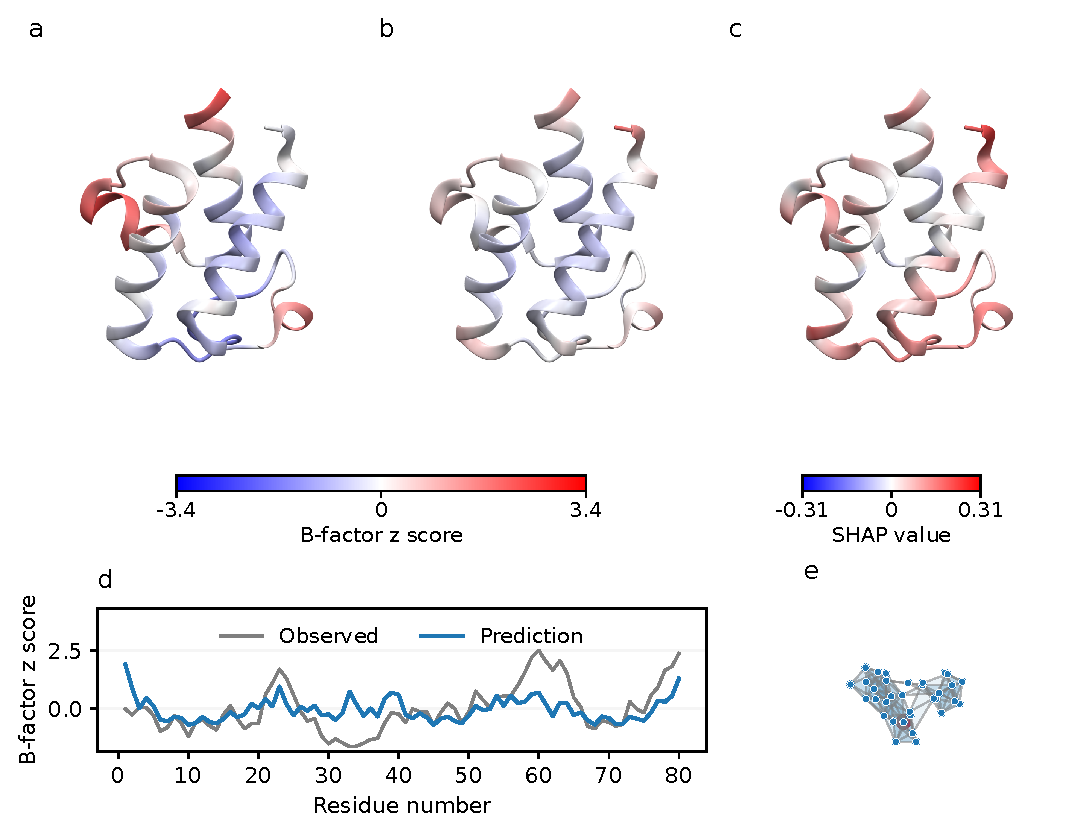
\includegraphics[width=\linewidth]{figures/supp_1X3O.pdf}
\caption{The predetermined companion protein 1X3O. (a,b) Observed within-protein normalized B-factor and the sequence-cluster-held-out graph-plus-center-zero prediction, mapped to the same residue coordinates and shown with a common color scale. (c) The signed sum of TreeSHAP contributions from the 24 center-zero spectral features, in B-factor z-score units. This subtotal excludes graph-feature contributions and the training-background expectation; blue is negative and red positive. (d) Observed and predicted residue profiles provide a direct check alongside the structural views. (e) The local alpha complex at ball radius 4~\AA\ within the fixed 13~\AA\ support of chain A residue 43. The protein, model protocol, and feature grouping were specified before inspecting prediction outcomes.}
\label{fig:companion}
\end{figure}

% Generated by scripts/summarize_study.py; do not transcribe historical metrics here.



\begin{table}[htbp]\centering\small
\caption{Degree-zero ablations of graph plus center-zero features. All models keep all graph features. The paired change is relative to the full multiscale spectral representation.}
\begin{tabular}{lrr}\toprule
Spectral summaries retained & Mean PCC [95\% CI] & Paired change [95\% CI]\\\midrule
Nullities only & 0.627 [0.613, 0.640] & -0.0005 [-0.0029, +0.0018] \\
Positive spectra only & 0.627 [0.613, 0.641] & -0.0000 [-0.0014, +0.0013] \\
Radius 3\,\AA & 0.628 [0.614, 0.641] & +0.0006 [-0.0015, +0.0026] \\
Radius 4\,\AA & 0.625 [0.611, 0.639] & -0.0025 [-0.0045, -0.0006] \\
Radius 5\,\AA & 0.628 [0.614, 0.641] & +0.0006 [-0.0016, +0.0028] \\
Radius 6\,\AA & 0.626 [0.612, 0.640] & -0.0011 [-0.0029, +0.0005] \\
\bottomrule\end{tabular}\end{table}




\begin{table}[htbp]\centering\small
\caption{Persistent-minus-static degree-one comparisons. All additions use twelve features on the same graph-plus-degree-zero baseline. Intervals are paired cluster-bootstrap intervals for mean protein PCC.}
\begin{tabular}{llr}\toprule
Sheaf & Static comparator & Paired PCC change [95\% CI]\\\midrule
Identity & Lower & -0.0004 [-0.0016, +0.0009] \\
Identity & Upper & +0.0000 [-0.0013, +0.0012] \\
Geometric & Lower & +0.0001 [-0.0011, +0.0012] \\
Geometric & Upper & +0.0011 [-0.0005, +0.0029] \\
Center-zero & Lower & +0.0004 [-0.0013, +0.0021] \\
Center-zero & Upper & -0.0005 [-0.0024, +0.0012] \\
\bottomrule\end{tabular}\end{table}




\begin{table}[htbp]\centering\small
\caption{Nonzero degree-one kernel frequencies across all 78,400 residue-centered neighborhoods. Neighborhoods are weighted equally. Identity and geometric nullities agree exactly at all evaluated scales. Equal endpoints describe the corresponding sheaf cohomology; unequal endpoints describe its persistent cohomology restriction rank.}
\begin{tabular}{lrrrr}\toprule
Radius pair (\AA) & \shortstack{Identity\\nonzero (\%)} & \shortstack{Center-zero\\nonzero (\%)} & \shortstack{Mean identity\\nullity} & \shortstack{Mean center\\nullity}\\\midrule
$(3,3)$ & 93.383 & 94.871 & 5.168 & 5.392 \\
$(4,4)$ & 83.679 & 86.844 & 3.102 & 3.488 \\
$(5,5)$ & 34.569 & 43.594 & 0.558 & 0.769 \\
$(6,6)$ & 3.221 & 6.657 & 0.039 & 0.080 \\
$(3,4)$ & 28.578 & 36.213 & 0.360 & 0.481 \\
$(5,6)$ & 0.361 & 2.140 & 0.004 & 0.022 \\
\bottomrule\end{tabular}\end{table}




\begin{table}[htbp]\centering\small
\caption{Protein-only split sensitivity analysis on the same 364 structures.}
\begin{tabular}{lrrr}\toprule
Representation & PCC [95\% CI] & Spearman & RMSE$_z$\\\midrule
Graph geometry & 0.622 [0.608, 0.636] & 0.602 & 0.789 \\
Legacy graph spectra & 0.609 [0.594, 0.623] & 0.598 & 0.848 \\
Graph + legacy spectra & 0.626 [0.612, 0.639] & 0.607 & 0.786 \\
Center-zero spectra & 0.560 [0.543, 0.576] & 0.554 & 0.877 \\
Graph + identity sheaf & 0.625 [0.611, 0.639] & 0.608 & 0.785 \\
Graph + geometric sheaf & 0.626 [0.612, 0.639] & 0.610 & 0.785 \\
Graph + center-zero sheaf & 0.624 [0.610, 0.638] & 0.608 & 0.786 \\
\bottomrule\end{tabular}\end{table}





\FloatBarrier
\subsection{Tracing claims to evidence}
\label{sec:evidence_details}
Every empirical number in the results is intended to trace to a current output table and its configuration. Cohort counts trace to the inclusion and fold manifests; prediction statistics trace to per-protein held-out metrics; uncertainty traces to the declared bootstrap; case-study claims trace to residue-keyed prediction and attribution rows. The manuscript uses generated numerical inputs for this reason. Citations to earlier PSL studies describe their published results and corrections, while mathematical statements are tied to the operators defined here. Neither an older manuscript's number nor an unverified biological narrative is evidence for a new result.

\section{Discussion}
\subsection{Representation complexity and biological information}
The principal empirical comparison limits the predictive claim supported by the center-zero construction. Mean protein PCC is \GraphPCC\ for graph geometry and \CombinedPCC\ after adding the degree-zero spectra, with paired increment $\DeltaPCC$ and 95\% interval $[\DeltaCILow,\DeltaCIHigh]$. The interval includes zero, so this experiment does not resolve a mean gain under the fixed evaluation. It also does not establish equivalence: small benefits and small losses remain compatible with that interval, and no equivalence margin was specified. The protein-only sensitivity analysis gives the same qualitative conclusion. Center-zero spectra alone perform less well than the graph baseline, emphasizing the need to assess incremental information against explicit geometric controls.

The mathematical analysis identifies information shared by spectra and simpler geometric descriptors. The native maximum records neighborhood size, its positive mean records neighbor-edge density, and other summaries retain graph organization beyond those counts. The center-zero degree-zero operator combines an inverse-square center packing term with the deletion graph's weighted spectrum. Both representations can therefore exploit local geometry already partly described by the graph features. Their small paired increments measure usefulness to the chosen forest. Representation independence and physical effects of the center label require separate tests.

Identity and all-one geometric additions have slightly higher mean PCC than the center-zero addition in this experiment, with positive paired intervals relative to graph alone. These exploratory comparisons motivate examining the restriction rule itself, including the coupling removed by a zero center. The predictive effect of localization by a label must be tested. The comparison remains conditional on the chosen summaries, scales, and regressor. The mathematical decomposition is useful regardless of which variant attains the largest point estimate: it identifies what was added and which simpler descriptors should be tested alongside it.

\subsection{What persistence can establish here}
Persistence is defined for a compatible pair of complexes and their maps. On a fixed vertex set, the degree-zero persistent upper operator is exactly the upper-endpoint graph operator. This redundancy follows directly from the operator definition. Testing persistence in this setting requires a degree where the lower complex omits cells present in the upper complex. In degree one, new edges create the constraint that distinguishes the Schur-complement operator from a static spectrum.

The degree-one comparisons do not resolve a predictive advantage of the persistent additions over either static endpoint control: every matched interval includes zero for identity, geometric, and center-zero sheaves. This result applies to the selected summaries and prediction task. Other uses of persistence require their own evaluation. The descriptor audit records different positive-spectrum summary vectors for most neighborhoods, even though those differences provide little resolved incremental value to the fitted forests. Algebraic distinctness and predictive usefulness are separate questions. The endpoint controls separate the effect of the pair operator from that of accessing larger-scale simplices.

The deletion/link characterization suggests more focused follow-up work than indiscriminate feature expansion. One can compare block-specific spectra, examine residues where center-link connectivity changes, or inspect the stability of the smallest positive eigenvalues under controlled coordinate perturbations. These hypotheses follow from the mathematics and remain to be tested. Any attempt to attribute a scalar eigenvalue to a particular molecular motion would require additional dynamical or physical evidence.

\subsection{Explanations at the level of residues}
The signed residue maps complement the mean comparison. A positive contribution from a sheaf scale can be offset by graph contributions, and the prediction combines both with its background expectation. Consequently, a striking local attribution remains compatible with a small mean incremental gain across proteins. Signed views and residue profiles preserve the direction of these contributions and expose prediction errors that an unsigned structural heat map could hide.

The decomposition describes the descriptor before fitting; SHAP describes how the fitted forest uses it. An exact spectral identity does not identify which summary the model uses, while a large attribution does not establish molecular mechanism. Their combination connects the representation's algebra to the model's behavior at an identified residue.

The images support statements about agreement with the crystallographic target and signed model contributions. Functional or dynamical interpretations would require independent residue-specific evidence. The companion protein supplies a second predetermined context and uses the same attribution definition and color scales.

\section{Limitations and reproducibility}
This study uses one historical structural collection and a coarse-grained coordinate representation. The observed \calpha\ sequence can omit disordered segments, and missing residues have no target row in the present analysis. The representation consequently describes the resolved portion of a deposited structure. Its coverage is limited by unresolved residues and the conditions of structure determination. B-factor normalization removes between-protein mean and scale, but it does not remove static disorder, crystal contacts, or refinement effects. An independent dynamics benchmark would be needed to assess prediction of motion in solution.

The sequence-cluster design reduces one form of train--test relatedness; it does not eliminate every dependency. Alignment thresholds are operational choices, observed-sequence coverage is affected by unresolved residues, and structures can share fold geometry without meeting the sequence rule. In particular, short-chain entries are protected against exact complete-sequence duplication but do not meet the 50-pair threshold for an alignment-based link. Small datasets also make feature comparisons sensitive to which clusters are difficult. Reporting the original and amended grouping graphs, the paired results, and the bootstrap intervals makes these effects inspectable. The reported evaluation remains conditional on this collection and split.

All spectral summaries are lossy. Distinct weighted complexes can be cospectral, and six summary statistics discard considerably more information than the full spectrum. Minimum positive eigenvalues also depend on numerical separation from zero, particularly for persistent operators formed by eliminating dependent directions. Degenerate geometries and floating-point rank decisions therefore require explicit checks. Our mathematical identities constrain the implementation, while the released diagnostics record their numerical realization.

The finite CPU budget limits the parameter grid and discourages an extensive search over radii, sheaf weights, and model hyperparameters. The timing pilot supported the full eligible cohort for the declared degree-one pairs, but this does not identify an optimal member of the entire descriptor family. Predictive comparisons should be read at that scope. Computational cost is reported as an experimental outcome because a small gain from a much more expensive representation may have a different practical value from the same gain using a simple graph summary.

The repository supplies scripts, configurations, residue and fold manifests, and tables tracing reported values to regenerated predictions. Figures use those same outputs. Source hashes identify third-party structures; historical result snapshots remain separate from the corrected experiment. These records make the representation, data-selection amendments, numerical decisions, and evaluation jointly inspectable.

\section{Conclusion}
The native center-labeled descriptor has an explicit weighted-graph spectrum, while the compatible center-zero sheaf separates deletion and augmented weighted-link contributions. Fixed support makes degree-zero persistence redundant with its upper endpoint and makes degree one the relevant setting for this persistence experiment. On the audited collection, the primary center-zero degree-zero increment is small and its paired interval includes zero. Degree-one persistence changes most spectral summary vectors but yields no resolved advantage over its static endpoint controls. These findings delimit predictive claims while providing an interpretable account of local sheaf spectra, supported by reproducible matrix checks, controlled experiments, and residue-level explanations tied to the evaluated model.

\section*{Data and code availability}
Code, exact configurations, generated metric tables, and figure sources for this study are available on the \href{https://github.com/ryan-charette/psl-protein-flexibility/tree/research-pivot}{research-pivot branch of the project repository}. The structural dataset is attributed to \citet{feng2025}; its recorded retrieval information and structure hashes accompany the data manifest. The extended derivations, implementation checks, detailed preprocessing policies, additional result tables, and companion visualization are integrated into this manuscript. The manuscript's numerical inputs are generated directly by the current analysis pipeline.

\bibliographystyle{unsrtnat}
\bibliography{references}
\end{document}
